\documentclass[12pt,oneside,a4paper]{report}
\usepackage{amsmath}
\usepackage{amssymb}
\usepackage[style=ieee]{biblatex}
\addbibresource{references.bib}
\usepackage{graphicx}
\usepackage{booktabs}
\usepackage{multirow}
\usepackage{lscape}
\usepackage{longtable}
\usepackage{textcomp}
\usepackage[margin=1in]{geometry}
\usepackage{float}
%% Times new roman font
%\usepackage{mathptmx}
%% Arial font
%\usepackage{helvet}
%\renewcommand{\familydefault}{\sfdefault}
\usepackage{hyperref}
\usepackage[all]{hypcap}
\title{Detecting abnormalities on chest X-rays using deep neural networks}
\author{
  Swaroop Kumar M L\\
  Department of Studies in Computer Science\\
  University of Mysore
}
\date{\today}
\linespread{1.25}
\begin{document}
\maketitle
\renewcommand\abstractname{\Large{\textbf{ABSTRACT}}}
\begin{abstract}
  \textbf{\textit{Diseases like pneumonia and tuberculosis are leading causes of
      death world-wide. Although conclusive diagnosis requires other tests such
      as a sputum culture, chest radiography can be an important diagnostic aid
      and is routinely recommended since it is fast, affordable and highly
      sensitive. Moreover, automated detection of abnormalities on the chest
      X-ray can help in active case finding, screening, and in cases where other
      tests are not available or are inconclusive. Due to the nature of the
      domain, it is also important that algorithms not only make inferences
      but also generate explanations sufficient to convince a human expert.}}\\

  \textbf{\textit{Inspired by previous work, we develop algorithms that can
      detect abnormalities on the x-ray. The algorithm explains these detections
      by generating heatmaps pointing out areas of the image that most
      influenced it. We establish baselines, benchmark against previous work and
      show that a) transfer-learning from a large non-TB dataset dramatically
      improves TB detection, b) models in the domain show inferior performance
      on external data from a different hospital system but c) recent techniques
      such as mixup and progressive resizing improve performance and
      generalization. We achieve performance competitive with previous work in
      detecting pneumonia-like and other abnormalities on the NIH chestX-ray14
      dataset and in detecting tuberculosis on the Shenzhen hospital dataset,
      and achieve state-of-the-art performance on the Montgomery county
      tuberculosis dataset. We look for potential sources of bias, test
      our baseline with respect to gender, age and view-position and evaluate
      our models on viral and bacterial pneumonia separately.}}
\end{abstract}
\tableofcontents
\listoftables
\listoffigures
\chapter{Introduction}
\section{Problem definition}
The lungs are made up of small air-sacks called alveoli. When, for example, air
in the alveoli is replaced with pus, blood and other fluids, referred to as
consolidation and commonly caused by pneumonia, or when abscesses in the lung
rupture forming cavities, indicating a tuberculosis infection, these are
visible on the chest x-ray. See figure \ref{basic_examples} for examples.\\

Radiologists are trained to look for signs of these abnormalities, use subtle
visual features to differentiate among the various types, reason about their
causes and help in diagnosis and treatment. An algorithm that can automatically
detect these abnormalities can be useful in numerous ways (see section
\ref{motivation}).\\
% \begin{enumerate}
% \item{Helping to actively find patients who may be infected with a particular
%   disease in the general population }
% \item{As an initial screening test before other, less affordable tests}
% \item{Prioritizing patients for subsequent review by a trained radiologist or
%   aiding a radiologist in other ways by being part of her workflow }
% \end{enumerate}
\begin{figure}
  % \fbox{
  % \begin{minipage}{\textwidth}
  \centering
  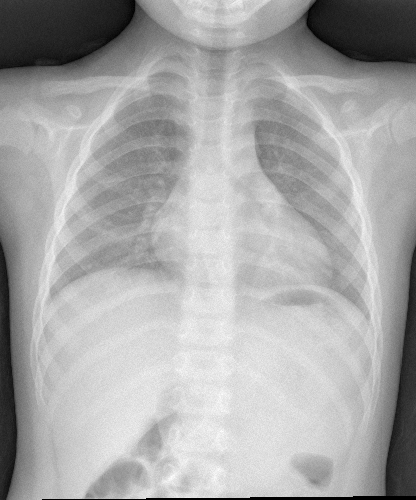
\includegraphics[width=0.3\textwidth]{images/normal1}\hspace{0.01\textwidth}%
  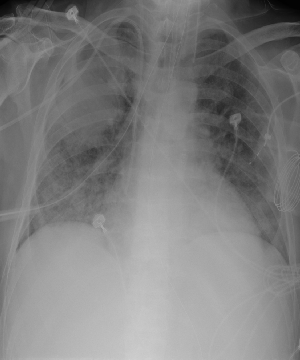
\includegraphics[width=0.3\textwidth]{images/consolidation_original}\hspace{0.01\textwidth}%
  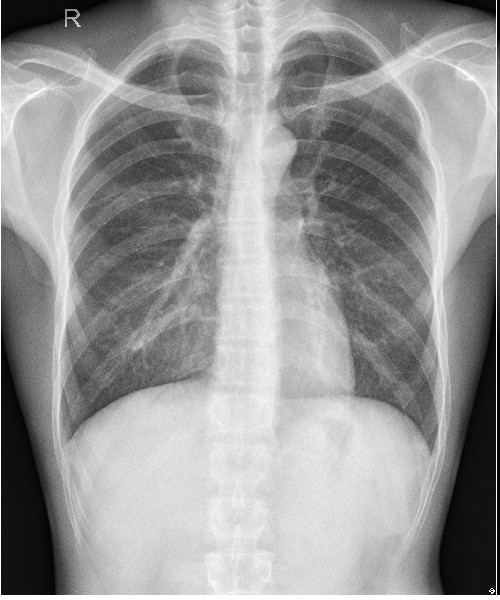
\includegraphics[width=0.3\textwidth]{images/TB_original}\\[0.01\textwidth]
  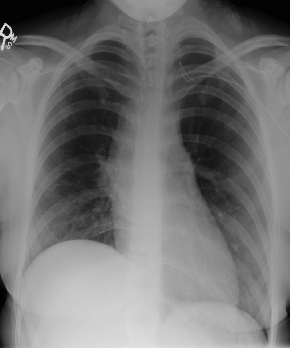
\includegraphics[width=0.3\textwidth]{images/normal2}\hspace{0.01\textwidth}%
  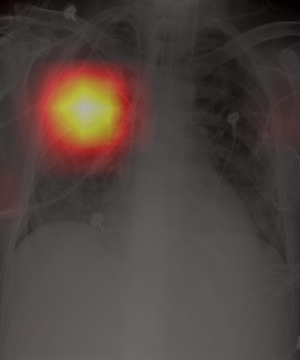
\includegraphics[width=0.3\textwidth]{images/consolidation_heatmap}\hspace{0.01\textwidth}%
  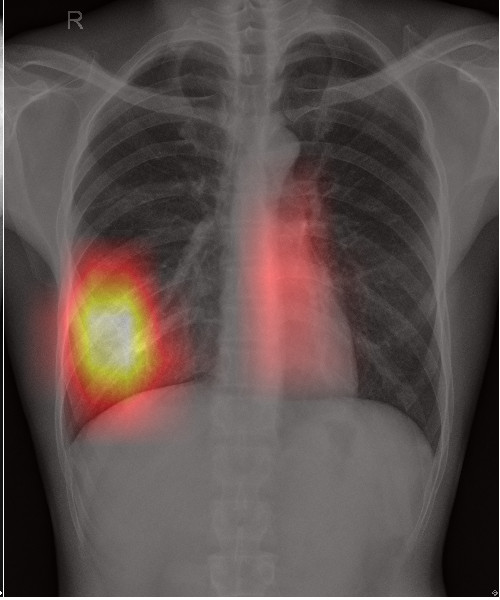
\includegraphics[width=0.3\textwidth]{images/TB_heatmap}
  \caption{From left to right: The first column shows two \emph{Normal} images.
    Columns 2 and 3 show images with \emph{Pneumonia} and \emph{Tuberculosis}
    respectively, the first row showing the original images and the second
    showing the same overlaid with heatmaps localizing the abnormalities, which
    we call \emph{explanations}}
  % \end{minipage}
  % }
  \label{basic_examples}
\end{figure}

However, building the hardware and software infrastructure for a clinically
relevant system that is useful in practice is a problem which presents unique
challenges of its own. Our work focuses on the core algorithm. We divide the
problem into, and explore, four sub-problems.
\subsection{Classification}
For our primary dataset, a large collection of chest x-rays annotated with
multiple abnormalities including pneumonia \cite{Wang2017a} (see section
\ref{nih_cxr}), we formulate the problem as a multi-class multi-label
classification problem. Given the $n$-dimensional input feature space $X =
\mathbb{R} ^n$, and a set of $c$ class labels corresponding to $c$ abnormalities
$L = \{\,l_1 ,l_2 ,l_3 \dots l_c\,\}$ the task is to learn a function $f:X
\rightarrow 2^L$ from the training set $D = \{\,(x_i, Y_i) \mid 1 \leq i \leq m
\,\}$. For each example $(x_i, Y_i) \in D$, $x_i \in X$ is an $n$-dimensional
feature vector $\{\, x_{i1}, x_{i2}, x_{i3} \dots x_{in} \,\}$, each feature
representing the intensity value of a single pixel of the input image, and $Y_i
\subseteq L $ is the set of abnormalities associated with $x_i$. For an unseen
instance $x$, the classifier $f(\cdot)$ predicts $f(x) \subseteq L$ as the set
of abnormalities for
$x$.\\

For the Shenzhen hospital tuberculosis dataset\cite{jaeger2014two} (see section
\ref{shenzhen}), we formulate the problem as a binary classification problem.
Again, suppose $X$ is the $n$-dimensional input feature space. The task is to
learn a function $f:X \rightarrow \{\,0, 1 \,\}$ from the training set $D =
\{\,(\,x_i, y_i) \mid 1 \leq i \leq m\,\}$. For each $(x_i, y_i) \in D$, $x_i
\in X$ is an $n$-dimensional feature vector $\{\,x_{i1}, x_{i2}, x_{i3} \dots
x_{in}\,\}$, each feature corresponding to the intensity value of a single pixel
of the input image, and $y_i \in \{\,0, 1\,\}$ is the corresponding label, $0$
meaning \emph{normal} and $1$ meaning \emph{tuberculosis}. Given an unseen $x
\in X$, the classifier
$f(\cdot)$ predicts $f(x) \in \{\,0, 1\,\}$ as being the label for $x$.\\

\subsection{Explainability}
Deep neural networks have outperformed previous methods in several domains.
However, they remain black-boxes with millions of parameters, leading to a lack
of trust and limiting their use in routine clinical practice. Several methods
have been proposed to make these models more interpretable, broadly falling into
two categories:
\begin{enumerate}
\item{Methods that create a proxy model which behaves similarly to the original
    model, but is simpler and easier to understand. These include methods like
    LIME\cite{ribeiro2016should} and SHAP\cite{NIPS2017_7062}. While these
    methods are model-independent, they tend to be very slow.}
\item{Methods that generate a saliency map which highlights a small portion of
    the input which is most relevant, in a single forward and backward pass
    through the network. These include methods like LRP\cite{bach2015pixel},
    DeepLIFT\cite{shrikumar2017learning}, CAM\cite{zhou2016learning} and
    Grad-CAM\cite{selvaraju2017grad}.}
\end{enumerate}
Given an input $x = \{\, x_{1}, x_{2}, x_{3} \dots x_{n} \,\} \in X$, and a set
of class labels $L = \{\,l_1 ,l_2 ,l_3 \dots l_c\,\}$, the task is to compute
the attribution
\begin{equation}
  A_j = \{\,a_{j1}, a_{j2}, a_{j3} \dots a_{jn}\,\} \in \mathbb{R} ^n
\end{equation}
for each class $l_j \in L$ where $a_{ji} \in A_j$ is a measure of the relevance
of
the $i^{th}$ feature to the model's inference regarding the $j^{th}$ class.\\

\subsection{Generalizability}
A test set is considered representative of data that will be encountered in the
external world and is used exclusively to evaluate a model. However, true
generalization to new datasets may be lower than expected.
\begin{enumerate}
\item{Since model design choices are based on previous work, methods in an
    application domain may overfit to one or a few popular datasets. However,
    \cite{recht2018cifar} shows that this is not the case for CIFAR-10 despite
    years of methods being tested on this dataset}
\item{Two datasets may have different distributions. In the context of
    biomedical imaging, datasets may be collected from different hospital
    systems and machines. For example, in \cite{zech2018variable}, Zech et al.
    show that models trained on data from one hospital system showed inferior
    performance on data from others.}
\item{The dataset used to train a model may have confounding variables that do
    not exist in other datasets. For example, in \cite{zech2018variable}, Zech
    et al. also show that CNNs were able to directly detect the hospital system
    and department within a hospital system from a chest radiograph where
    saliency maps showed high activation in image corners. We observed the same
    phenomenon in networks that were trained to detect abnormalities. Since
    different departments and machines within a hospital system have different
    prevalence of a disease, the model may leverage these spurious correlations
    and fail to generalize.}
\end{enumerate}
Therefore, it is important that models are evaluated on external datasets from
different hospital systems.

\subsection{Fairness}
Machine learning systems are increasingly being deployed in settings where they
may inadvertently learn and leverage biases in the datasets, discriminate based
on race, gender, etc. and amplify existing social inequities. For example, in
\cite{bolukbasi2016man}, Bolukbasi et al. show that the popular word embedding
space Word2Vec encodes gender bias. In \cite{buolamwini2018gender}, Buolamwini
et al. show that facial recognition datasets are overwhelmingly composed of
light-skinned individuals and that commercial gender classification systems
performed worse for dark-skinned people and females, with a difference in
accuracy of more than 30\% between
light-skinned males and dark-skinned females.\\

There has been substantial work in the research literature on fairness in ML on
the development of statistical definitions of fairness
\cite{chouldechova2017fair,dwork2012fairness,hardt2016equality} and algorithmic
methods to measure and mitigate undesirable biases
\cite{agarwal2018reductions,hardt2016equality,kusner2017counterfactual}. A
simple measure against bias in various fields has been to hide variables like
gender and race from a model, but complex machine learning models learn to use
other correlated variables as proxy for hidden ones (for example, zipcode as
correlated with race and the word `women' in an institution's name as correlated
with the gender of its students\cite{dastin_2018}). Moreover, hiding sensitive
variables from researchers exacerbates the problem by limiting their ability to
quantify and mitigate these biases. For example, in
\cite{esteva2017dermatologist}, Estava et al. found that convolutional neural
networks are effective at detecting melanoma from images. However, without
labels for skin characteristics such as color, accuracy of the
model for different skin-types cannot be measured.\\

We measure the potential for discrimination by
training models with architectures similar to the abnormality detection model,
to identify gender and age group from images alone.
We then test our baseline model's performance across genders and age groups.

\section{Motivation\label{motivation}}
Pneumonia and tuberculosis are leading causes of death worldwide. According to
the world health organization, pneumonia disproportionately affects children,
accounting for 16\% of all deaths of children under the age of 5
years\cite{who_pneumonia}. Tuberculosis is more prevalent in countries where
many people live in absolute poverty\cite{tb_poverty} with limited access to
healthcare and in 2017 alone, caused 1.6
million preventable deaths\cite{who_tb}.\\

The global End TB strategy aims for a 95\% reduction in deaths due to TB by 2035
compared with 2015. Similarly, the National Strategic Plan (NSP) 2017-2025 sets
out to achieve a rapid decline in deaths due to TB and emphasizes the importance
of active case finding, that is, detection of TB cases early by seeking out
people in targeted groups and scaling up cheap and high sensitivity TB
diagnostic tests. The NSP has recommended three tests: sputum smear microscopy,
chest x-ray and the new CB-NAAT\footnote{CB-NAAT or Cartridge Based Nucleic Acid
  Amplification Test is a molecular test and is
  known as GeneXpert outside India} test.\\

Conventionally, patients are screened for TB or pneumonia related symptoms,
sputum examinations are recommended for those with positive symptoms, and chest
x-rays are recommended for those who test negative in the sputum examination.\\

With automated detection, x-ray tests have the potential to be faster and
significantly more affordable. They can be massively scaled up and used
\begin{enumerate}
\item{For active case finding in high-risk populations, for example, with mobile
    x-ray vans\cite{modi_suresh_2019}}
\item{As an initial screening test before or along with other tests such as a
    sputum examination}
\item{To aid a radiologist in her workflow by sorting her queue based on
    severity, suggesting areas to consider in an image, providing a second
    opinion, etc.}
\end{enumerate}

Our goal is to make automated abnormality detection systems such as ours more
clinically relevant and trust-worthy by a) improving their accuracy and
explainability, b) evaluating their ability to generalize to other hospital
systems and c) exploring the potential for algorithms in this domain to be
unfair.
\section{Previous work}
In \cite{Wang2017}, Wang et al. collect chest x-ray images and their associated
reports from the PAC system of the National Institutes of Health and mine labels
from the reports algorithmically. They evaluate the accuracy
of these labels and establish a baseline for abnormality detection.\\

Previous work has explored methods to improve classification performance. In
\cite{Guan2018,Tang2018,Wang2018b,Pesce2017}, the authors use attention-guided
learning to allow a network to concentrate on abnormal regions of the image.
\cite{Tang2018} also uses curriculum learning and presents images in increasing
order of difficulty. However, \cite{Cai2018} uses attention to hide the most
salient regions, allowing the network to pay attention to other areas.
\cite{Yao,Wang2018b} seek to exploit correlations between abnormalities,
\cite{Yao} by using an LSTM and \cite{Wang2018b} by extracting saliency maps at
an intermediate layer and providing these as input to subsequent layers.\\

There has also been work on improving localization by combining feature maps
from multiple layers of the network \cite{Yao2018a,Sedai2018}. \cite{Sedai2018}
learns a set of \emph{layer relevance weights} for each class, and
\cite{Yao2018a} applies a DenseNet per resolution orthogonal to a standard
ResNet followed by upsampling and concatenation.\\

In \cite{Rajpurkar2018}, Rajpurkar et al. train a variant of DenseNet on the NIH
chestX-ray14 dataset relabeled using an ensemble of classifiers and report
super-human performance for several abnormalities, comparing board-certified
radiologists and the algorithm on a test set labeled by consensus of three
cardiothoracic subspeciality radiologists. Both Wang et al. in \cite{Wang2017}
and Rajpurkar et al. in \cite{Rajpurkar2018} use weakly supervised localization
to explain the
network's inference.\\

For TB detection, previous work such as \cite{Jaeger2014,Lopes2017,Vajda2018}
have explored various feature extraction techniques, feature selection
strategies and classifiers such as logistic regression and SVM.
\cite{Hwang2016,Islam2017,Haloi2018a,Liu2018} train deep convolutional neural
networks and ensemble these. These methods have also explored the usefulness of
segmentation of chest regions. Due to the lack of large publicly available
datasets, work in this domain, especially the application of deep learning
methods, has been limited. Moreover, results are less relevant to clinical
practice as models trained on small two-class datasets are prone to over-diagnose.\\

We apply methods proposed by \cite{VanNoord2017,Zhang2017}. In
\cite{VanNoord2017}, van Noord et al. propose a multi-scale CNN which learns
both scale-variant and scale-invariant features at an artist attribution task.
In \cite{Zhang2017}, Zhang et al. introduce a technique called \emph{mixup} and
show that it improves generalization and helps to mitigate the negative effects
of label noise.
\section{Our work}
We use a 121-layer dense convolutional network
\emph{DenseNet}\cite{huang2017densely}. The network's connectivity pattern
improves the flow of information and gradients
and has fewer parameters, making it possible to train very deep networks.\\

For the NIH chestX-ray14 dataset of 112,120 x-ray images of 30,805 unique
patients labeled with up-to 14 different abnormalities, we randomly split the
dataset into a training set, a validation set and a test set, consisting of
roughly 70\%, 10\% and 20\% of the patients respectively. We replace the final
fully-connected layer of the network with one that has 14 outputs after which we
apply a sigmoid non-linearity. The output of the network is a 14-dimensional
vector $P = \{\,p_1, p_2, p_3 \dots p_{14}\,\}$ where $p_k \in P$ corresponds to
the $k^{th}$ abnormality and $0 \leq p_k \leq 1$. Using the
Adam\cite{kingma2014adam} optimization algorithm, we optimize the sum of binary
cross entropy losses
\begin{equation}
  l(x, Y) = \sum_{k=1} ^{14}[-y_k\log p_k-(1-y_k)\log (1-p_k)]
\end{equation}
where $(x, Y)$ is a pair in the training set and $y_k$ is 1 if $Y$ contains the
$k^{th}$ abnormality and 0 otherwise.
% \begin{equation}
%   y_k =
%   \begin{cases}
%     1 & \text{if $l_k \in Y$}\\
%     0 & \text{otherwise}
%   \end{cases}
% \end{equation}
A set of optimal thresholds $T = \{\,t_1, t_2, t_3 \dots t_{14}\,\}$ is
determined by maximizing the network's F1-score on the training set and applied
to the output of the network. Given an unseen image $x$, the output of the
network is $P = \{\,p_1, p_2, p_3 \dots p_{14}\,\}$ and the final output $Y
\subseteq L$ after applying the thresholds is:
\begin{equation}
  Y = \{\,l_i \in L \mid p_i \in P \wedge t_i \in T \wedge p_i > t_i \,\}
\end{equation}

Similarly, for the Shenzhen hospital tuberculosis dataset with 662 frontal chest
x-ray images, we create 9 folds of the dataset and report the mean and standard
deviation of performance. We replace the final fully-connected layer of the
network with one that has 2 outputs after which we apply a sigmoid
non-linearity. The output of the network is a 2-dimensional vector $P = \{\,p_1,
p_2\,\}$ where $0 \leq p_1 \leq 1$ and $0 \leq p_2 \leq 1$. Using the Adam
optimization algorithm, we optimize the binary cross entropy loss
\begin{equation}
  l(x, y) = -y\log p_2-(1-y)\log (1-p_1)]
\end{equation}
where $(x, y)$ is a pair in the training set. Given an unseen image $x$, the
output of the network is $P = \{\,p_1, p_2\,\}$ and the final output $y$ is 1
(tuberculosis) if $p2 >
p1$ and 0 (normal) otherwise.\\
% \begin{equation}
%   y = 
%   \begin{cases}
%     0 & \text{if $p1 \geq p2$\, (normal)}\\
%     1 & \text{if $p2 > p1$\, (tuberculosis)}
%   \end{cases}
% \end{equation}

The network consists of a fully convolutional backbone followed by an
adaptive-average-pooling layer and a single fully-connected layer. The fully
convolutional part of the network results in $k$ $w$ x $h$ feature maps which
are averaged along the width and height to form a $k$ dimensional vector, which
is fed to the single fully-connected layer with $k$ input nodes and $c$ output
nodes. If $f_i$ is the $i^{th}$ feature map and $w^j _i$ is the weight between
the $i^{th}$ input node and the $j^{th}$ output node in the fully-connected
layer, the saliency map for the $j^{th}$ class $M_j$ is
\begin{equation}
  M_j = \sum _i \, w^j _i \, f_i
\end{equation}
$M_j$ is a $w$ x $h$ saliency map which is interpolated to the size of the input
image and measures the relevance of each pixel to the model's decision regarding
the $j^{th}$ class, and can be visualized as a heatmap (see figure
\ref{basic_examples}). This serves as an \emph{explanation} of the model's
inference, allowing physicians and radiologists to decide how much trust to
invest in it.\\

To test the ability of these networks to generalize to other hospital systems,
we use two external datasets, a pediatric pneumonia dataset with 5332 x-ray
images\cite{kermany2018identifying} and a smaller tuberculosis dataset of 138
frontal chest x-ray images\cite{jaeger2014two}.\\

We evaluate the potential for bias by training similar networks to predict the
gender and age group of a patient and the view-position (AP vs. PA) given only
the x-ray image and evaluate our baseline for each gender, age group and view
position.\\

We make the following observations:
\begin{enumerate}
\item{ On the NIH chestX-ray14 dataset, using only horizontal flipping for data
    augmentation led to overfitting but extending this to include rotation,
    zooming, brightness scaling and perspective warp reduced overfitting and
    improved performance. Also, a recently proposed data augmentation technique,
    mixup\cite{Zhang2017}, consistently improved performance on both internal
    and external datasets.}

\item{ Compared to random initialization, initializing the weights of all but
    the final layers of the network with those of a similar network trained on a
    large collection of natural images, ImageNet, significantly improved
    performance. }

\item{ At the problem of tuberculosis detection, pre-training on the NIH
    chestX-ray14 dataset significantly improved performance and generalization
    to the external dataset. However, this lead to over-diagnosis of TB on the
    NIH chestX-ray14 dataset. }

\item{ Training a single network on 224 x 224 images until the validation loss
    plateaued and repeatedly re-training it on progressively higher resolution
    images improved generalization to external datasets, as did preserving these
    intermediate models and ensembling them\cite{VanNoord2017}.}

\item{ Models trained to detect Tuberculosis on the Shenzhen dataset showed
    inferior performance on the Montgomery county dataset, and models trained to
    detect pneumonia and other abnormalities on the NIH chestX-ray14 dataset
    performed worse on the external dataset than a similar network trained
    exclusively on the smaller external dataset. }

\item{For most abnormalities, average saliency maps or explanations weighted by
    predicted probability, of models trained on the NIH chestX-ray14 dataset
    showed high activation at image corners, predominantly the top-left and
    top-right, on both the internal and external datasets. However, cropping of
    image margins at both training and inference stages, did not negate this
    effect. }
  
\item{ Baselines showed similar performance for each gender, age group and
    view-position. However, networks with architecture similar to the
    abnormality detection network, after a single epoch of training were able to
    distinguish between x-ray images of male and female patients and determine
    the view-position with more than 90\% accuracy. }

\item{Models trained on the NIH CXR-14 dataset were better at
	detecting viral pneumonia than bacterial pneumonia.}

\end{enumerate}\\

For the Shenzhen tuberculosis dataset, pre-training on the NIH chestX-ray14
dataset resulted in an AUC of 98.4\% and an accuracy of 94.6\% which are
respectively 2.8\% and 4.4\% better than our baseline. On the external dataset,
the same model achieves an AUC of 95.5\% and accuracy of 89.4\% which are
respectively 8.1\% and 15.2\% better than our baseline. On both the Shenzhen and
Montgomery datasets, our model is competitive with previous work and
out-performs previous works that use deep neural networks.\\

On the NIH chestX-ray14 dataset, training a single network on 224 x 224 images,
repeatedly re-training on progressively higher resolution images, preserving
these intermediate models and ensembling them resulted in an average AUC of
85.6\% which is 1.8\% better than our baseline and competitive with previous
work. This translated to a 3.6\% improvement on the pediatric pneumonia
dataset.\\

% \section{Report layout}


\chapter{Data\label{data}}
We use the NIH ChestX-ray14 dataset\cite{Wang2017} and the Shenzhen hospital
tuberculosis dataset\cite{jaeger2014two} to train models to detect pneumonia and
other abnormalitites, and tuberculosis respectively. We then use two external
datasets, the Guangzhou medical center pediatric pneumonia
dataset\cite{kermany2018identifying} and the Montgomery county tuberculosis
dataset\cite{jaeger2014two} as \emph{external} datasets to test the ability of
these models to generalize to other hospital systems.

\begin{table}[]
  \centering
  \begin{tabular}{@{}llll@{}}
    \toprule
    \textbf{}                              & \textbf{Training} & \textbf{Testing} & \textbf{\begin{tabular}[c]{@{}l@{}}Different\\ Hospital system?\end{tabular}} \\ \midrule
    \multirow{3}{*}{\textbf{Pneumonia}}    & NIH CXR-14        & NIH CXR-14       & No                                                                            \\ \cmidrule(l){2-4} 
                                           & NIH CXR-14        & Guangzhou   & Yes                                                                           \\ \cmidrule(l){2-4} 
                                           & Guangzhou    & Guangzhou   & No                                                                            \\ \midrule
    \multirow{3}{*}{\textbf{Tuberculosis}} & Shenzhen          & Shenzhen         & No                                                                            \\ \cmidrule(l){2-4} 
                                           & Shenzhen          & Montgomery       & Yes                                                                           \\ \cmidrule(l){2-4} 
                                           & Montgomery        & Montgomery       & No                                                                            \\ \bottomrule
  \end{tabular}
  \caption{Datasets used for training and testing}
  \label{tab:test-combos}
\end{table}

\section{NIH CXR-14\label{nih_cxr}}
The NIH chestX-ray14 dataset consists of 112,120 chest x-ray images of 30,805
unique patients which was collected using the PAC system of the National
Institutes of Health. Each image was labeled with up-to 14 abnormalities
algorithmically using the associated radiology report in natural language.\\

About half or 60,361 of these are labeled as \emph{No finding} and the rest are
labeled with one of more of the 14 abnormalities. Some abnormalities are more
common than others, the most common being \emph{Infiltration}, which is present
in 19,894 images, and the least common being \emph{Hernia}, which is present in
only 227 images.\\

We split the dataset into train, validation and test sets roughly in the ratio
70:10:20. We make sure that there is no patient overlap, that is, all images of
a patient are in the same subset since patient overlap may lead to overfitting.

\begin{table}[]
  \centering
  \begin{tabular}{@{}lllll@{}}
    \toprule
    \textbf{Abnormality} & \multicolumn{4}{l}{\textbf{Number of images}}        \\ \midrule
                         & Train     & Validation & Test      & Total           \\ \midrule
    Atelectasis          & 7996      & 1119       & 2420      & 11559           \\ \midrule
    Cardiomegaly         & 1950      & 240        & 582       & 2776            \\ \midrule
    Effusion             & 9261      & 1292       & 2754      & 13317           \\ \midrule
    Infiltration         & 13914     & 2018       & 3938      & 19894           \\ \midrule
    Mass                 & 3988      & 625        & 1133      & 5782            \\ \midrule
    Nodule               & 4375      & 613        & 1335      & 6331            \\ \midrule
    Pneumonia            & 978       & 133        & 242       & 1431            \\ \midrule
    Pneumothorax         & 3705      & 504        & 1089      & 5302            \\ \midrule
    Consolidation        & 3263      & 447        & 957       & 4667            \\ \midrule
    Edema                & 1690      & 200        & 413       & 2303            \\ \midrule
    Emphysema            & 1799      & 208        & 509       & 2516            \\ \midrule
    Fibrosis             & 1158      & 166        & 362       & 1686            \\ \midrule
    Pleural Thickening   & 2279      & 372        & 734       & 3385            \\ \midrule
    Hernia               & 144       & 41         & 42        & 227             \\ \midrule
    No Finding           & 42405     & 6079       & 11928     & 60361           \\ \midrule
    \textbf{Total}       & \textbf{78468} & \textbf{11219}  & \textbf{22433} & \textbf{112120} \\ \bottomrule
  \end{tabular}
  \caption{For the NIH CXR-14 dataset, the number of images in the train,
    validation and test sets per abnormality}
  \label{tab:nih_split}
\end{table}

\subsection{Challenges and issues}
The NIH chestX-ray14 dataset is one of the largest publicly accessible chest
x-ray datasets. However, it presents a few unique challenges:
\begin{enumerate}
\item{\textbf{Noisy labels}\\
    Labels were extracted using NLP from radiology reports in natural language
    text. This may lead to label noise. \cite{Wang2017} show that these labels
    are about 90\% accurate. Although deep neural networks have been shown to be
    robust to label noise in general\cite{rolnick2017deep}, structured noise can
    be especially detrimental to performance.}
\item{\textbf{Labeling schema}\\
    Some of these abnormalities are sub-types of others, but labels are provided
    as a non-hierarchical list. For example, \emph{Pneumonia} on the x-ray is a
    form of \emph{Consolidation} }
\item{\textbf{Class imbalance}\\
    The majority of images do not contain abnormalities, and some abnormalities
    are common while others are rare. For example, \emph{Infiltration} appears
    in 17\% of the images while \emph{Hernia} appears in only 0.2\% of the images.}
\end{enumerate}

\section{Guangzhou\label{mendeley}}
The Guangzhou pediatric pneumonia dataset consists of 8,497 chest x-ray images
of children under the age of 5 years collected from the Guangzhou Women and
Children’s Medical Center, Guangzhou. Each image has been labeled as either
\emph{Normal} (4232 images) or \emph{Pneumonia} (4265 images). Images labeled as
\emph{Pneumonia} have been further tagged as \emph{Bacterial} (2772
images) or \emph{Viral} (1493 images) based on the cause of pneumonia.\\

We use the standard test set and split the rest of the dataset into train and
validation sets in the ratio 80:20.
However, when used as an external dataset, we use the entire dataset.\\

\begin{table}[]
  \centering
  \begin{tabular}{@{}lllll@{}}
    \toprule
    \textbf{Label}      & \multicolumn{4}{l}{\textbf{Number of images}}  \\ \midrule
                        & Train     & Validation & Test      & Total     \\ \midrule
    Normal              & 3199      & 799        & 234       & 4232           \\ \midrule
    Viral pneumonia     & 1076      & 269        & 148       & 1493          \\ \midrule
    Bacterial pneumonia & 2024      & 506        & 242       & 2772          \\ \midrule
    \textbf{Total}      & \textbf{6299} & \textbf{1574}  & \textbf{624} & \textbf{8497} \\ \bottomrule
  \end{tabular}
  \caption{For the Guangzhou pediatric pneumonia dataset, the number of images
    in the train, validation and test sets per label}
  \label{tab:guangzhou_split}
\end{table}

\section{Shenzhen\label{shenzhen}}
The Shenzhen tuberculosis dataset consists of 615 chest x-ray images collected
from the Shenzhen No.3 Hospital in Shenzhen, Guangdong providence, China. Each
of the images is labeled as either \emph{Normal} or \emph{Tuberculosis}. 340 of
these are normal and 275 show manifestations of tuberculosis.\\

Considering the small size of the dataset, we create 9 folds of the dataset and
report average and standard deviation of metrics. Each fold contains all the
images split into train, validation and test sets in the ratio 70:10:20.\\

\begin{landscape}
  \begin{table}[]
    \centering
    \begin{tabular}{@{}lllllllllll@{}}
      \toprule
      \textbf{Label}                & \textbf{Set} & \multicolumn{9}{l}{\textbf{Number of images}}                                                                        \\ \midrule
                                    &              & Fold 1    & Fold 2    & Fold 3    & Fold 4    & Fold 5    & Fold 6    & Fold 7    & Fold 8    & Fold 9        \\ \midrule
      \multirow{3}{*}{Normal}       & Train        & 220       & 220       & 220       & 211       & 211       & 211       & 222       & 222       & 222                 \\ \cmidrule(l){2-11} 
                                    & Validation   & 28        & 39        & 39        & 39        & 38        & 38        & 39        & 31        & 34                  \\ \cmidrule(l){2-11} 
                                    & Test         & 78        & 67        & 67        & 76        & 77        & 77        & 65        & 73        & 70                  \\ \midrule
      \multirow{3}{*}{Tuberculosis} & Train        & 222       & 222       & 222       & 231       & 231       & 231       & 220       & 220       & 220                 \\ \cmidrule(l){2-11} 
                                    & Validation   & 45        & 34        & 35        & 33        & 35        & 36        & 34        & 42        & 40                  \\ \cmidrule(l){2-11} 
                                    & Test         & 69        & 80        & 79        & 71        & 70        & 69        & 82        & 74        & 76                  \\ \bottomrule 
    \end{tabular}
    \caption{For the Shenzhen tuberculosis dataset, the number of images in the
      train, validation and test sets in each fold per label}
    \label{tab:shenzhen_split}
  \end{table}
\end{landscape}

\section{Montgomery\label{montgomery}}
The Montgomery county tuberculosis dataset consists of 138 chest x-ray images
collected from the tuberculosis control program of the Department of Health and
Human Services of Montgomery County, MD, USA. Each of the images is labeled as
either \emph{Normal} or \emph{Tuberculosis}. 80 of these are normal and 58 show manifestations of tuberculosis. The dataset also contains manually segmented lung masks for each image.\\

Similar to the Shenzhen dataset, we create 9 folds and report average and
standard deviation of metrics. Each fold contains all the images split into
train, validation and test sets in the ratio 70:10:20. However, when used as an
external dataset, we ignore these folds and test on the
entire dataset.\\

\begin{landscape}
  \begin{table}[]
    \centering
    \begin{tabular}{@{}lllllllllll@{}}
      \toprule
      \textbf{Label}                & \textbf{Set} & \multicolumn{9}{l}{\textbf{Number of images}}                                                                        \\ \midrule
                                    &              & Fold 1    & Fold 2    & Fold 3    & Fold 4    & Fold 5    & Fold 6    & Fold 7    & Fold 8    & Fold 9        \\ \midrule
      \multirow{3}{*}{Normal}       & Train        & 55        & 55        & 55        & 53        & 53        & 53        & 52        & 52        & 52                  \\ \cmidrule(l){2-11} 
                                    & Validation   & 8         & 7         & 10        & 9         & 9         & 9         & 11        & 8         & 9                   \\ \cmidrule(l){2-11} 
                                    & Test         & 17        & 18        & 15        & 18        & 18        & 18        & 17        & 20        & 19                  \\ \midrule
      \multirow{3}{*}{Tuberculosis} & Train        & 37        & 37        & 37        & 39        & 39        & 39        & 40        & 40        & 40                  \\ \cmidrule(l){2-11} 
                                    & Validation   & 7         & 8         & 6         & 6         & 6         & 7         & 4         & 7         & 7                   \\ \cmidrule(l){2-11} 
                                    & Test         & 14        & 13        & 15        & 13        & 13        & 12        & 14        & 11        & 11                  \\ \bottomrule
    \end{tabular}
    \caption{For the Montgomery county tuberculosis dataset, the number of
      images in the train, validation and test sets in each fold per label}
    \label{tab:mc_split}
  \end{table}
\end{landscape}

\chapter{Baselines\label{baselines}}
\section{Model architecture\label{architecture}}
We replace the final fully connected layer of 121-layer dense convolutional
neural network with one that has either 14 outputs (for the NIH CXR-14 dataset)
or 2 outputs (for all other datasets) after which we apply a sigmoid
non-linearity. The fully convolutional backbone of the network results in $k$
$w$ x $h$ feature maps and is followed by a global-average-pooling layer where
the $k$ feature maps are averaged along the width and height to form a $k$
dimensional vector. This makes the network independent of input image size and
allows us to use the
progressive-resizing method (see section \ref{progressive_resizing}).\\

The network's connectivity pattern improves the flow of information and
gradients and has fewer parameters, making it possible to train very deep
networks. The architecture of the model, specifically the fact that the fully
convolutional part of the network is followed by a single fully connected layer,
forces the model to learn to localize abnormalities given only weak labels (presence or absence of an abnormality).\\

\begin{figure}
  \centering 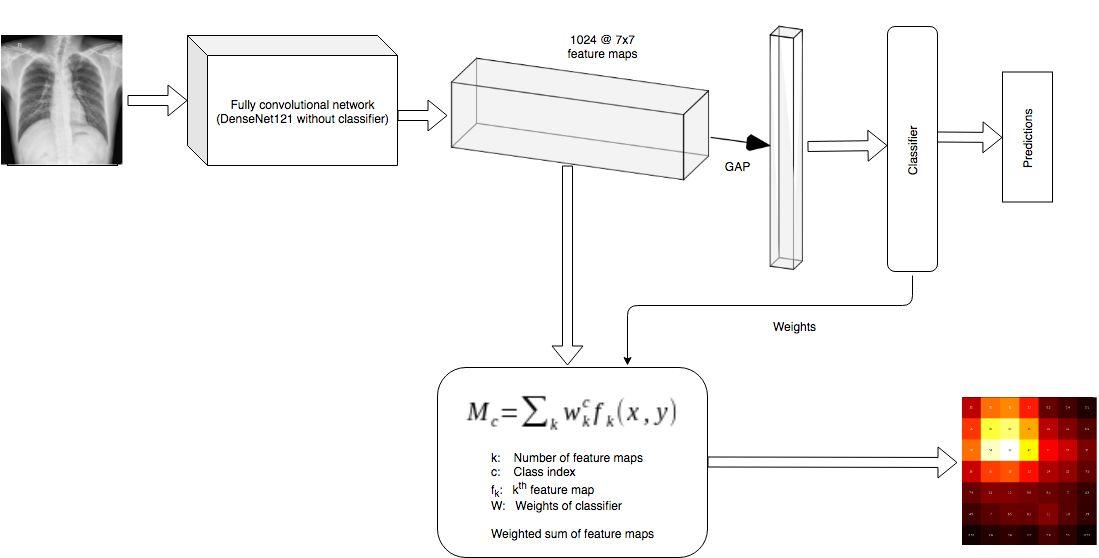
\includegraphics[width=\textwidth]{images/arch}
  \caption{Basic architecture of the model}
  \label{architecture}
\end{figure}

\section{Training procedure\label{training_procedure}}
We use the Adam optimization algorithm and start the training with an initial
learning rate a factor of 10 smaller than the learning rate at which the
training loss begins to increase, when the learning rate is increased linearly
(using a learning rate finder). We divide the learning rate by 10 if the
validation loss plateaus (does not decrease over 5 iterations), and stop
training when the validation loss has stopped decreasing. When using k-fold
cross validation, we train $k$ different networks on each of the $k$ folds and
report average and standard deviation
of performance.\\

\section{Inference procedure\label{inference_procedure}}
At the multi-class multi-label classification task (for the NIH CXR-14 dataset),
we merge the train and validation sets after training and use it to compute
optimal thresholds for each abnormality by optimizing for the class-specific
F1-score. Although it is possible to compute optimal thresholds for the
classification task since we have ground truth labels, it is not possible to do
so for the localization task since
we only have weak labels and not precise locations.\\

At binary classification tasks, since the network has two output nodes, we do
not compute thresholds but simply consider as the proper output the class whose
corresponding output node has higher activation.

\section{Saliency maps and bounding boxes}
To compute explanations, we save the feature maps resulting from the final
convolutional layer during a forward pass and perform a weighted sum of these
feature maps using the weights of the final fully-connected layer between
each of the feature maps and the desired output node, as follows.\\

If $f_i$ is the $i^{th}$ feature map and $w^j _i$ is the weight between the
$i^{th}$ input node and the $j^{th}$ output node in the fully-connected layer,
the saliency map for the $j^{th}$ class $M_j$ is
\begin{equation}
  M_j = \sum _i \, w^j _i \, f_i
\end{equation}
$M_j$ is a $w$ x $h$ saliency map which we interpolate to the size of the input
image and visualize as a heatmap (see figure \ref{basic_examples}).\\

We use a region-growing algorithm to determine bounding boxes given a saliency
map. Specifically, we first threshold the saliency map and using the maximum
element as a seed point, grow a region around it, including all non-zero
neighbours, and repeat the same until all non-zero elements are included in a
region, each time choosing as seed the maximum element not included a region.
For each region, we determine a bounding box as the smallest rectangle which
encloses the entire region. For example, see figure \ref{cam_bbox_examples}

\begin{figure}
  \centering
  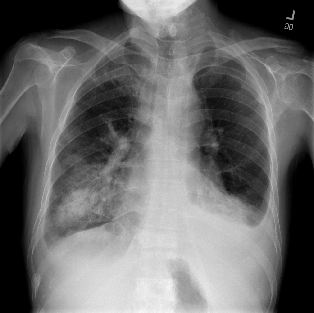
\includegraphics[width=0.45\textwidth]{images/pneumonia_orig}\hspace{0.01\textwidth}%
  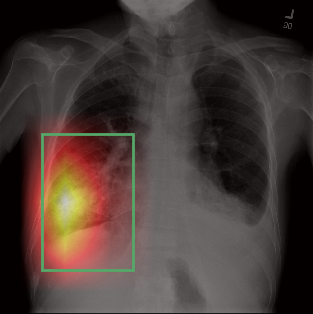
\includegraphics[width=0.45\textwidth]{images/pneumonia_hm_bbox}\\[0.01\textwidth]
  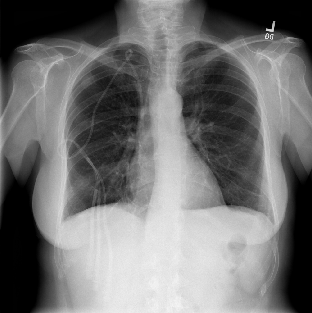
\includegraphics[width=0.45\textwidth]{images/atelectasis_orig}\hspace{0.01\textwidth}%
  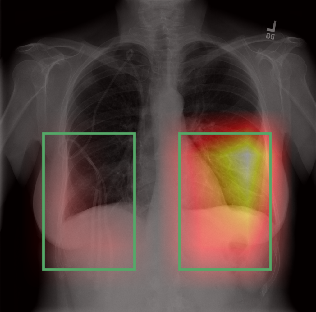
\includegraphics[width=0.45\textwidth]{images/atelectasis_hm_bbox}\\[0.01\textwidth]
  \caption{Examples of saliency maps with corresponding bounding boxes drawn.
    The first column shows original x-ray images and the second row shows
    saliency map and bounding boxes overlaid on the image. Row 1: Pneumonia. Row
    2: Atelectasis.}
  \label{cam_bbox_examples}
\end{figure}

\section{Evaluation metrics}
We primarily use the area under the reciever-operator-characteristic curve
(AUROC) to measure the performance of a model. AUROC is not affected by the
class distribution, does not need thresholds to be set, and is commonly used in
the literature. Apart from AUROC and accuracy, we also use

\begin{enumerate}
\item{\textbf{Specificity}\\
    Specificity is a measure of the model's ability to reject negative examples.
    \begin{equation}
      Specificity = \frac{|TN|}{|TN| + |FP|}
    \end{equation}
  }
\item{\textbf{Sensitivity}\\
    Sensitivity is a measure of the model's ability to detect positive examples.
    \begin{equation}
      Sensitivity = \frac{|TP|}{|TP| + |FN|}
    \end{equation}
  }
\end{enumerate}
Where $|TP|$ is the number of true positives, $|TN|$ is the number of true
negatives, $|FP|$ is the number of false positives and $|FN|$ is the number of
false negatives.

\section{Baseline performance}
Training on 224 x 224 images of the NIH CXR-14 dataset using a batch size of 16,
initial learning rate of 0.01, momentum of 0.9, weight decay of $10^{-5}$ and
horizontal flipping (with a probability of 0.5) as data augmentation, we obtain
average AUROC (of 14 abnormalities) of 0.838 which is competitive with previous
work. Results are shown in table \ref{tab:baseline_nih}.\\

Training on 224 x 224 images of the Shenzhen hospital tuberculosis dataset with
a batch size of 16, initial learning rate of 0.0001, momentum of 0.9, weight
decay of $10^{-5}$ and using random horizontal flipping (with a probability
0.5), random rotation (0\textdegree{} to 10\textdegree{}), random zoom (1x to
1.1x), random brightness scaling(upto 1.2x with a probability of 0.75) and
random perspective warping as data augmentation, we obtain an average AUROC (of
9 folds) of 0.956 with a standard deviation of 0.009, which is
competitive with previous work using similar methods. Results are shown in
table \ref{tab:baseline_shenzhen}.\\

\begin{table}[]
  \centering
  \begin{tabular}{@{}ll@{}}
    \toprule
    \textbf{Abnormality} & \textbf{AUROC} \\ \midrule
    Atelectasis          & 0.823          \\ \midrule
    Cardiomegaly         & 0.905          \\ \midrule
    Effusion             & 0.879          \\ \midrule
    Infiltration         & 0.712 	  \\ \midrule
    Mass                 & 0.839          \\ \midrule
    Nodule               & 0.778   	  \\ \midrule
    Pneumonia            & 0.760          \\ \midrule
    Pneumothorax         & 0.869          \\ \midrule
    Consolidation        & 0.806 	  \\ \midrule
    Edema                & 0.891          \\ \midrule
    Emphysema            & 0.923          \\ \midrule
    Fibrosis             & 0.831 	  \\ \midrule
    Pleural Thickening  & 0.785          \\ \midrule
    Hernia               & 0.929          \\ \midrule
    \textbf{Average}     & \textbf{0.838}          \\ \bottomrule
  \end{tabular}
  \caption{Baseline results on the NIH CXR-14 dataset}
  \label{tab:baseline_nih}
\end{table}

\begin{table}[]
  \centering
  \begin{tabular}{@{}lllll@{}}
    \toprule
    & \textbf{AUROC} & \textbf{Accuracy} & \textbf{Specificity} & \textbf{Sensitivity} \\ \midrule
    Mean               & 0.956          & 0.902             & 0.902                & 0.899                \\ \midrule
    Standard deviation & 0.009          & 0.019             & 0.050                & 0.045                \\ \bottomrule
  \end{tabular}
  \caption{Baseline results on the Shenzhen hospital tuberculosis dataset}
  \label{tab:baseline_shenzhen}
\end{table}

\chapter{Experiments\label{exp}}
\section{Data augmentation}
We observe that the baseline model for the NIH CXR-14 dataset began to overfit
after about 20,000 iterations and the validation loss began to increase, as
shown in figure \ref{data_augmentation_loss}. However, adding more data
augmentation, random rotation (0\textdegree{} to 10\textdegree{}), random zoom
(1x to 1.1x), random brightness scaling(upto 1.2x with a probability of 0.75)
and random perspective warping in addition to horizontal flipping, the model did
not overfit upto 70,000 iterations and showed improvement in performance. Data
augmentation has the additional benefit of making the model more robust to
similar augmentations
during inference.\\

\begin{figure}
  \centering
  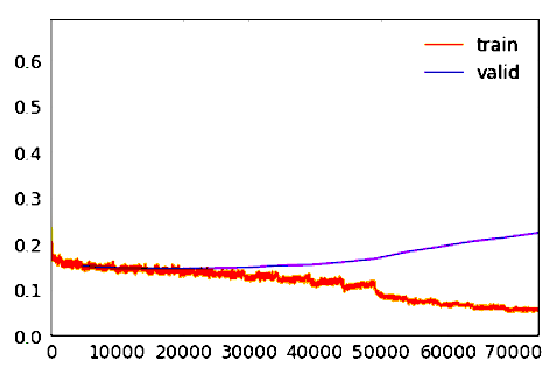
\includegraphics[width=0.49\textwidth]{images/baseline_without_da}\hspace{0.01\textwidth}%
  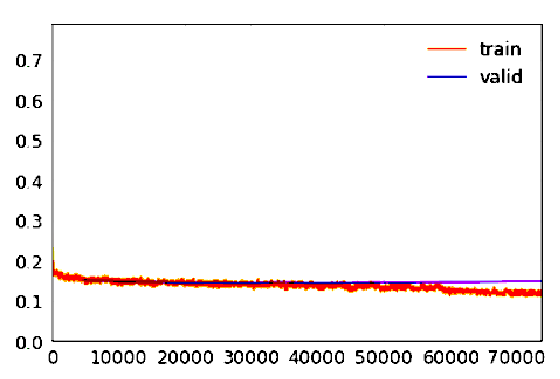
\includegraphics[width=0.49\textwidth]{images/baseline_with_da}\\[0.01\textwidth]
  \caption{Number of iterations (x-axis) vs training and validation loss
    (y-axis), with only horizontal flipping (left), and more data augmentations
    (right).}
  \label{data_augmentation_loss}
\end{figure}

\begin{table}[]
  \centering
  \begin{tabular}{@{}lll@{}}
    \toprule
    \textbf{Abnormality} & \multicolumn{2}{l}{\textbf{AUROC}}                                  \\ \midrule
    \textbf{}            & \textbf{Only horizontal flipping} & \textbf{More data augmentation} \\ \midrule
    Atelectasis          & 0.823                             & \textbf{0.826}                  \\ \midrule
    Cardiomegaly         & 0.905                             & \textbf{0.907}                  \\ \midrule
    Effusion             & 0.879                             & \textbf{0.884}                  \\ \midrule
    Infiltration         & \textbf{0.712}                    & 0.704                           \\ \midrule
    Mass                 & 0.839                             & \textbf{0.849}                  \\ \midrule
    Nodule               & \textbf{0.778}                    & 0.773                           \\ \midrule
    Pneumonia            & 0.760                             & \textbf{0.764}                  \\ \midrule
    Pneumothorax         & 0.869                             & \textbf{0.877}                  \\ \midrule
    Consolidation        & \textbf{0.806}                    & 0.799                           \\ \midrule
    Edema                & 0.891                             & \textbf{0.901}                  \\ \midrule
    Emphysema            & 0.923                             & \textbf{0.925}                  \\ \midrule
    Fibrosis             & \textbf{0.831}                    & 0.828                           \\ \midrule
    Pleural Thickening  & 0.785                             & \textbf{0.795}                  \\ \midrule
    Hernia               & 0.929                             & \textbf{0.949}                  \\ \midrule
    \textbf{Average}     & 0.838                             & \textbf{0.841}                  \\ \bottomrule
  \end{tabular}
  \caption{Results on the NIH CXR-14 dataset with and without additional data
    augmentations}
  \label{tab:da_vs_noda}
\end{table}
 
\section{Test-time augmentation}
We apply test-time augmentation and perform a weighted average of the model's
output on 5 different crops of the image (center and 4 corners) as well as the
horizontally flipped versions of each corner. We weight the center-crop by a
factor $\beta$ and each of the other augmentations with a weight
$\frac{1-\beta{}}{8}$.\\

Using a $\beta$ of 0.4, we find that performance consistently decreases across
abnormalities. See table \ref{tab:tta} for the results.

\begin{table}[]
  \centering
  \begin{tabular}{@{}lll@{}}
    \toprule
    \textbf{Model}                                                                                                      & \multicolumn{2}{l}{\textbf{Average AUROC}} \\ \midrule
                                                                                                                        & Without TTA          & With TTA            \\ \midrule
    Baseline                                                                                                            & \textbf{0.838}       & 0.829               \\ \midrule
    More data augmentation                                                                                              & \textbf{0.841}       & 0.838               \\ \midrule
    Higher resolution (512 x 512)                                                                                       & \textbf{0.836}       & 0.834               \\ \midrule
    Progressive resizing (upto 512 x 512)                                                                               & \textbf{0.846}       & 0.838               \\ \midrule
    \begin{tabular}[c]{@{}l@{}}Mixup with $\alpha$ = 1 (224 x 224)\\ Only horizontal flipping\end{tabular} & \textbf{0.834}       & 0.825               \\ \midrule
    Mixup with $\alpha$ = 1 (224 x 224)                                                                    & \textbf{0.852}       & 0.851               \\ \midrule
    Mixup with $\alpha$ = 0.4 (224 x 224)                                                                  & 0.849                & \textbf{0.850}      \\ \midrule
    Mixup with $\alpha$ = 0.4 (512 x 512)                                                                  & 0.852                & 0.852               \\ \bottomrule
  \end{tabular}
  \caption{Results on the NIH CXR-14 dataset with and without test-time
    augmentation}
  \label{tab:tta}
\end{table}

\section{Mixup}
Mixup is a recently proposed data augmentation technique \cite{Zhang2017} that
is effective at regularizing models. It has also been shown to combat label
noise and improve the model's ability to generalize. Instead of using raw
images, we feed the model a linear combination of two images not necessarily
from the same class. If $I_1$ and $I_2$ are two images, we feed the network a
linear combination $M = t \cdot{}I_1 + (1 - t) \cdot{}I_2$ where $t$ is drawn
from a beta distribution parameterized by some $\alpha$. The expected output for
$M$ is $ t \cdot{} y_1 + (1 - t) \cdot{} y_2$ where $y_1$ and $y_2$ are the
targets for $I_1$
and $I_2$ respectively.\\

Mixup improved performance on both the NIH CXR-14 dataset and the Shenzhen
tuberculosis dataset. It also improved generalization to external datasets.

\begin{table}[]
  \centering
  \begin{tabular}{@{}lllll@{}}
    \toprule
    \textbf{Training set}       & \textbf{Testing set}        & \textbf{Model}                                                   & \textbf{Average AUROC} &                \\ \midrule
                                &                             &                                                                  & Without mixup          & With mixup     \\ \midrule
    \multirow{5}{*}{NIH CXR-14} & \multirow{3}{*}{NIH CXR-14} & Baseline                                                         & \textbf{0.838}         & 0.834          \\ \cmidrule(l){3-5} 
                                &                             & \begin{tabular}[c]{@{}l@{}}More DA\\ (224 x 224)\end{tabular}      & 0.841                  & \textbf{0.852} \\ \cmidrule(l){3-5} 
                                &                             & \begin{tabular}[c]{@{}l@{}}More DA\\ (512 x 512)\end{tabular}      & 0.836                  & \textbf{0.852} \\ \cmidrule(l){2-5} 
                                & \multirow{2}{*}{Guangzhou}  & \begin{tabular}[c]{@{}l@{}}More DA\\ (224 x 224)\end{tabular}      & 0.842                  & \textbf{0.873} \\ \cmidrule(l){3-5} 
                                &                             & \begin{tabular}[c]{@{}l@{}}More DA\\ (512 x 512)\end{tabular}      & 0.818                  & \textbf{0.831} \\ \midrule
    \multirow{6}{*}{Shenzhen}   & \multirow{3}{*}{Shenzhen}   & (448 x 448)                                                      & 0.954                  & \textbf{0.956} \\ \cmidrule(l){3-5} 
                                &                             & \begin{tabular}[c]{@{}l@{}}(224 x 224)\\ Pretrained\end{tabular} & 0.977                  & \textbf{0.979} \\ \cmidrule(l){3-5} 
                                &                             & \begin{tabular}[c]{@{}l@{}}(480 x 480)\\ Pretrained\end{tabular} & 0.984                  & \textbf{0.985} \\ \cmidrule(l){2-5} 
                                & \multirow{3}{*}{Montgomery} & (448 x 448)                                                      & 0.809                  & \textbf{0.824} \\ \cmidrule(l){3-5} 
                                &                             & \begin{tabular}[c]{@{}l@{}}(224 x 224)\\ Pretrained\end{tabular} & 0.941                  & \textbf{0.947} \\ \cmidrule(l){3-5} 
                                &                             & \begin{tabular}[c]{@{}l@{}}(480 x 480)\\ Pretrained\end{tabular} & \textbf{0.957}         & 0.955          \\ \bottomrule
  \end{tabular}
  \caption{Results of mixup. Mixup consistently improves performance and
    generalization to external datasets.}
  \label{tab:mixup}
\end{table}

\section{Transfer-learning from ImageNet}
We initialize the weights of a network with those of a similar network trained
on a large dataset of millions of natural images, ImageNet and compare this with
random initialization (we use the Kaiming He initialization method\cite{he2015delving}).\\

We observe that pre-training on ImageNet significantly improves performance on
both internal and external datasets. See table \ref{tab:imagenet_pretraining}
for the results.

\begin{table}[]
  \centering
  \begin{tabular}{@{}lllll@{}}
    \toprule
    \textbf{Training set}       & \textbf{Testing set}        & \textbf{Model}                                                                   & \textbf{Average AUROC}                                                       &                                                                           \\ \midrule
                                &                             &                                                                                  & \begin{tabular}[c]{@{}l@{}}Without\\ pre-training\\ on ImageNet\end{tabular} & \begin{tabular}[c]{@{}l@{}}With\\ pre-training\\ on ImageNet\end{tabular} \\ \midrule
    \multirow{4}{*}{NIH CXR-14} & \multirow{2}{*}{NIH CXR-14} & \begin{tabular}[c]{@{}l@{}}More DA\\ (224 x 224)\end{tabular}                    & 0.794                                                                        & \textbf{0.841}                                                            \\ \cmidrule(l){3-5} 
                                &                             & \begin{tabular}[c]{@{}l@{}}More DA\\ (512 x 512)\end{tabular}                    & 0.791                                                                        & \textbf{0.836}                                                            \\ \cmidrule(l){2-5} 
                                & \multirow{2}{*}{Guangzhou}  & \begin{tabular}[c]{@{}l@{}}More DA\\ (224 x 224)\end{tabular}                    & 0.817                                                                        & \textbf{0.842}                                                            \\ \cmidrule(l){3-5} 
                                &                             & \begin{tabular}[c]{@{}l@{}}More DA\\ (512 x 512)\end{tabular}                    & 0.768                                                                        & \textbf{0.818}                                                            \\ \midrule
    \multirow{6}{*}{Shenzhen}   & \multirow{3}{*}{Shenzhen}   & \begin{tabular}[c]{@{}l@{}}More DA\\ (224 x 224)\end{tabular}                    & 0.894                                                                        & \textbf{0.956}                                                            \\ \cmidrule(l){3-5} 
                                &                             & \begin{tabular}[c]{@{}l@{}}More DA\\ (672 x 672)\end{tabular}                    & 0.876                                                                        & \textbf{0.960}                                                            \\ \cmidrule(l){3-5} 
                                &                             & \begin{tabular}[c]{@{}l@{}}Progressive\\ resizing\\ up-to 672 x 672\end{tabular} & 0.902                                                                        & \textbf{0.954}                                                            \\ \cmidrule(l){2-5} 
                                & \multirow{3}{*}{Montgomery} & \begin{tabular}[c]{@{}l@{}}More DA\\ (224 x 224)\end{tabular}                    & 0.596                                                                        & \textbf{0.871}                                                            \\ \cmidrule(l){3-5} 
                                &                             & \begin{tabular}[c]{@{}l@{}}More DA\\ (672 x 672)\end{tabular}                    & 0.583                                                                        & \textbf{0.813}                                                            \\ \cmidrule(l){3-5} 
                                &                             & \begin{tabular}[c]{@{}l@{}}Progressive\\ resizing\\ up-to 672 x 672\end{tabular} & 0.617                                                                        & \textbf{0.829}                                                            \\ \bottomrule
  \end{tabular}
  \caption{Results of pre-training on ImageNet. Pre-training on Imagenet, a
    large collection of natural images, significantly improves both performance
    and generalization}
  \label{tab:imagenet_pretraining}
\end{table}

\section{Transfer-learning from NIH CXR-14}
On the Shenzhen hospital tuberculosis dataset, we compare replacing the weights
of a network with those of a similar network a) trained on ImageNet (a large
non-x-ray dataset of natural images) and b) trained on ImageNet and then on NIH
CXR-14 (a smaller non-tb x-ray
dataset).\\

We observe that pre-training on the NIH CXR-14 dataset both improves performance
on both the internal test set and helps to close the generalization gap (see
table \ref{tab:pretraining_nih}).

\begin{table}[]
  \centering
  \begin{tabular}{@{}llllll@{}}
    \toprule
    \textbf{Test set} & \textbf{Model}                                                                    & \multicolumn{2}{l}{\textbf{AUROC}}                                            & \multicolumn{2}{l}{\textbf{Accuracy}}                                         \\ \midrule
                      &                                                                                   & Mean           & \begin{tabular}[c]{@{}l@{}}Standard\\ deviation\end{tabular} & Mean           & \begin{tabular}[c]{@{}l@{}}Standard\\ deviation\end{tabular} \\ \midrule
    Shenzhen          & Baseline                                                                          & 0.956          & 0.009                                                        & 0.902          & 0.019                                                        \\ \midrule
                      & \begin{tabular}[c]{@{}l@{}}Pre-trained on\\ NIH CXR-14\\ (224 x 224)\end{tabular} & 0.977          & 0.006                                                        & 0.934          & 0.017                                                        \\ \midrule
                      & \begin{tabular}[c]{@{}l@{}}Pre-trained on\\ NIH CXR-14\\ (480 x 480)\end{tabular} & \textbf{0.984} & \textbf{0.006}                                               & \textbf{0.946} & \textbf{0.015}                                               \\ \midrule
    Montgomery        & Baseline                                                                          & 0.871          & 0.029                                                        & 0.755          & 0.038                                                        \\ \midrule
                      & \begin{tabular}[c]{@{}l@{}}Pre-trained on\\ NIH CXR-14\\ (224 x 224)\end{tabular} & 0.941          & 0.014                                                        & 0.860          & 0.030                                                        \\ \midrule
                      & \begin{tabular}[c]{@{}l@{}}Pre-trained on\\ NIH CXR-14\\ (480 x 480)\end{tabular} & \textbf{0.957} & \textbf{0.012}                                               & \textbf{0.890} & \textbf{0.019}                                               \\ \bottomrule
  \end{tabular}
  \caption{Results of pre-training on NIH CXR-14. Pre-training networks on the
    NIH CXR-14 14 improves performance on both the internal test set and the
    external dataset}
  \label{tab:pretraining_nih}
\end{table}

\section{Overdiagnosis of TB}
The rate of of tuberculosis in the NIH CXR-14 dataset is unknown since
tuberculosis is not one of the labels. However, assuming a baseline rate of less
than 1\%, we observe that models trained to detect tuberculosis on the Shenzhen
hospital tuberculosis dataset tend to over-diagnose when tested on the NIH
CXR-14 dataset.\\

The rate of over-diagnosis is especially high when models are pre-trained on the
NIH CXR-14 dataset. However, models trained using progressive resizing without
pre-training on the NIH CXR-14 dataset have the lowest rate of over-diagnosis
(see table \ref{tab:overdiagnosis}).
\begin{table}[]
  \centering
  \begin{tabular}{@{}ll@{}}
    \toprule
    \textbf{Model}                                                                    & \textbf{Over-diagnosis (\%)} \\ \midrule
    Baseline                                                                          & 8.5                          \\ \midrule
    \begin{tabular}[c]{@{}l@{}}Pre-trained on\\ ImageNet\\ (448 x 448)\end{tabular}   & 7.9                          \\ \midrule
    \begin{tabular}[c]{@{}l@{}}Pre-trained on\\ ImageNet\\ (672 x 672)\end{tabular}   & 14.5                         \\ \midrule
    \begin{tabular}[c]{@{}l@{}}Pre-trained on\\ NIH CXR-14\\ (224 x 224)\end{tabular} & \textbf{45.5}                \\ \midrule
    \begin{tabular}[c]{@{}l@{}}Pre-trained on\\ NIH CXR-14\\ (480 x 480)\end{tabular} & \textbf{36}                  \\ \midrule
    \begin{tabular}[c]{@{}l@{}}Progressive resizing\\ up-to (448 x 448)\end{tabular}  & 1.1                          \\ \midrule
    \begin{tabular}[c]{@{}l@{}}Progressive resizing\\ up-to (672 x 672)\end{tabular}  & 3.7                          \\ \bottomrule
  \end{tabular}
  \caption{Results of over-dianosis. Models trained on the Shenzhen dataset to
    detect tuberculosis tend to over-diagnose TB on the NIH CXR-14 dataset}
  \label{tab:overdiagnosis}
\end{table}
\section{Progressive resizing\label{progressive_resizing}}
For the NIH CXR-14 dataset dataset, we first train on 224 x 224 images until the
validation loss plateaus. We then re-train the same network on 256 x 256 images,
288 x 288 images, etc. upto 512 x 512 with a smaller learning rate and for
fewer epochs. The intuition behind progressive resizing is that first training
on lower resolution images is equivalent to pre-training and is better than
training on high resolution images from scratch. It may also make networks more
robust to scale variation and behave similar to
data augmentation preventing overfitting.\\

For the Shenzhen hospital tuberculosis dataset, we first train on 224 x 224
images, until the validation loss plateaus, and retrain the same network on 448
x 448 images and then on 672 x 672 images.\\

We observe that progressive resizing consistently improves performance and
generalization to external datasets. See table \ref{tab:progressive_resizing}
for the results.
\begin{table}[]
  \centering
  \begin{tabular}{llll}
    \hline
    \textbf{Internal dataset} & \textbf{External dataset} & \multicolumn{2}{l}{\textbf{AUROC}} \\ \hline
                              &                           & Without PR     & With PR           \\ \hline
    NIH CXR-14                & NIH CXR-14                & 0.836          & \textbf{0.846}    \\ \hline
                              & Gaungzhou                 & 0.818          & \textbf{0.871}    \\ \hline
    Shenzhen                  & Shenzhen                  & 0.96            & 0.954             \\ \hline
                              & Montgomery                & 0.813          & \textbf{0.829}    \\ \hline
  \end{tabular}
  \caption{Results for progressive resizing.}
  \label{tab:progressive_resizing}
\end{table}
\section{Ensembling predictions}
We ensemble the predictions from multiple models trained on different
resolutions using progressive resizing. This is similar to \cite{VanNoord2017},
the intuition being that scale-invariance emerges from ensembling.\\

We observe that ensembling improves performance across abnormalitites on the NIH
CXR-14 dataset and improves generalization to the Guangzhou dataset. It also
improves performance on the Shenzhen dataset for tuberculosis detection but
fails to generalize to the Montgomery dataset.
\begin{table}[]
  \centering
  \begin{tabular}{llll}
    \hline
    \textbf{Internal dataset} & \textbf{External dataset} & \multicolumn{2}{l}{\textbf{AUROC}} \\ \hline
                              &                           & Baseline         & Ensemble        \\ \hline
    NIH CXR-14                & NIH CXR-14                & 0.838            & \textbf{0.856}  \\ \hline
                              & Gaungzhou                 & 0.842            & \textbf{0.878}  \\ \hline
    Shenzhen                  & Shenzhen                  & 0.956            & \textbf{0.963}  \\ \hline
                              & Montgomery                & \textbf{0.871}   & 0.663           \\ \hline
  \end{tabular}
  \caption{Results for ensembling of predictions of multiple models trained
    using progressive resizing on different resolutions}
  \label{tab:ensembling}
\end{table}
\section{Ensembling saliency maps}
At the problem of tuberculosis detection, we experiment with ensembling saliency
maps from multiple models trained on different resolutions after interpolating
these to the size of the largest saliency map. Predictions are derived from the
saliency maps by using averaging across the width and height.\\

We observe that this method results in performance similar to ensembling final
predictions.

\section{Cropping of image margins}
For most models, saliency maps showed high activation at image corners when
detecting abnormalities, perhaps due to the presence of tokens on the x-ray
which differ between hospital systems and departments, and which may be
correlated with abnormalities. \cite{Zech2018} makes the same observation with
models trained to identify the hospital system from x-ray images. We experiment
with cropping out the top, bottom, left and right margins of the image. However,
average saliency maps still showed high activation in image corners. Figure
\ref{avg_saliency_maps} shows average saliency maps of pneumonia weighted by
predicted
probabilities for various models.\\

\begin{figure}[H]
  % \fbox{
  % \begin{minipage}{\textwidth}
  \centering
  \emph{a} 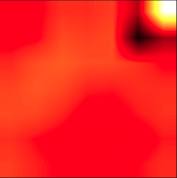
\includegraphics[width=0.28\textwidth]{images/heatmap_224_noda}\hspace{0.01\textwidth}%
  \emph{b} 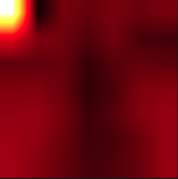
\includegraphics[width=0.28\textwidth]{images/heatmap_224_da}\hspace{0.01\textwidth}%
  \emph{c} 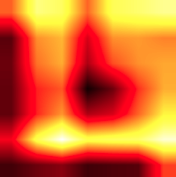
\includegraphics[width=0.28\textwidth]{images/heatmap_224_cropped}\\[0.01\textwidth]
  \hspace{0\textwidth}
  \emph{e} 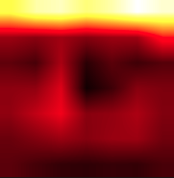
\includegraphics[width=0.28\textwidth]{images/heatmap_224_no_in}\hspace{0.01\textwidth}%
  \emph{d} 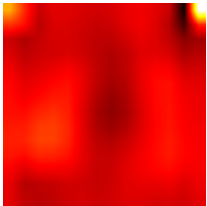
\includegraphics[width=0.28\textwidth]{images/heatmap_224_guangzhou}\hspace{0.15\textwidth}\\[0.01\textwidth]
  \caption{Average saliency maps for \emph{pneumonia}. Clockwise from the
    top-left: a) Baseline, b) Baseline with more data augmentation, c) Trained
    with margins cropped, d) Trained on NIH CXR-14, tested on Guangzhou and e)
    Trained without pre-training on ImageNet }
  % \end{minipage}
  % }
  \label{avg_saliency_maps}
\end{figure}


\section{Fairness}
% On the NIH CXR-14 dataset, we train a network similar to ours to identify
% gender, view position (AP vs. PA) and age-group from chest x-rays. We find that
% similar after one epoch of training, models can identify gender and view
% position from x-ray images with more that 90\% accuracy.\\

% We then measure performance of our model for each gender and view position. We
% find that the model shows similar performance for each gender and view position
% across abnormalities.

% \begin{table}[]
%   \centering
%   \begin{tabular}{lllll}
%     \hline
%     \textbf{Abnormality} & \textbf{Male : Female} & \multicolumn{3}{l}{\textbf{AUROC}}         \\ \hline
%                          &                        & Male                                                 & Female         & Both         \\ \hline
%     Atelectasis          & 1435:987               & \textbf{0.824}                                       & 0.820          & 0.829        \\ \hline
%     Cardiomegaly         & 290:292                & \textbf{0.894}                                       & 0.888          & 0.901        \\ \hline
%     Effusion             & 1517:1238              & \textbf{0.881}                                       & 0.875          & 0.888        \\ \hline
%     Infiltration         & 2332:1612              & 0.713                                                & \textbf{0.716} & 0.706        \\ \hline
%     Mass                 & 687:451                & 0.847                                                & \textbf{0.858} & 0.831        \\ \hline
%     Nodule               & 802:535                & 0.782                                                & \textbf{0.788} & 0.772        \\ \hline
%     Pneumonia            & 125:135                & 0.767                                                & \textbf{0.783} & 0.760        \\ \hline
%     Pneumothorax         & 537:552                & \textbf{0.871}                                       & 0.853          & 0.887        \\ \hline
%     Consolidation        & 553:404                & \textbf{0.800}                                       & 0.797          & 0.804        \\ \hline
%     Edema                & 214:199                & 0.897                                                & \textbf{0.905} & 0.890        \\ \hline
%     Emphysema            & 301:208                & \textbf{0.916}                                       & 0.902          & 0.933        \\ \hline
%     Fibrosis             & 211:151                & 0.825                                                & \textbf{0.845} & 0.798 \\ \hline
%     Pleural Thickening  & 473:261                & \textbf{0.768}                                       & 0.767          & 0.768 \\ \hline
%     Hernia               & 11:31                  & \textbf{0.922}                                       & 0.836          & 0.953 \\ \hline
%   \end{tabular}
%   \caption{Number of images of males and females and model performance across
%     abnormalities for each gender}
%   \label{tab:fairness}
% \end{table}

We look for potential sources of bias such as gender, age and view-position
by a) looking at the distribution of ground truth by gender, age and view-position and variable rates of abnormalities, b) training models with architecture similar to our baseline model to predict these from images alone. We then measure variable performance of our baseline model across gender, age-group and view-position.

\begin{table}[]
  \centering
  \begin{tabular}{@{}lllll@{}}
    \toprule
               & \textbf{Number of images} &          &        & \textbf{Rate of abnormality}                    \\ \midrule
               & Total            & Abnormal & Normal & \\ \midrule
Male           & 56804            & 26368    & 30436  & 0.464               \\
Female         & 44097            & 20200    & 23897  & 0.458               \\ \midrule
0 to 9 years   & 1214             & 470      & 744    & 0.387               \\
10 to 19 years & 4883             & 2036     & 2847   & 0.417               \\
20 to 29 years & 11575            & 4952     & 6623   & 0.428               \\
30 to 39 years & 14515            & 5971     & 8544   & 0.411               \\
40 to 49 years & 19543            & 8635     & 10908  & 0.442               \\
50 to 59 years & 24949            & 11976    & 12973  & 0.480               \\
60 to 69 years & 17500            & 8996     & 8504   & 0.514               \\
70 to 79 years & 5691             & 2946     & 2745   & 0.518               \\
80 to 89 years & 978              & 562      & 416    & 0.575               \\
90 to 99 years & 39               & 17       & 22     & 0.436               \\ \midrule
PA             & 60463            & 25179    & 35284  & 0.416               \\
AP             & 40438            & 21389    & 19049  & 0.529               \\
\bottomrule
\end{tabular}
\caption{Distribution of \emph{normal} and \emph{abnormal} images by gender, age group and view-position.}
\label{tab:distribution_overall}
\end{table}


\subsection{Age}
Age follows a rougly gaussian distribution with a mean of 46.17 years and standard deviation of 16.73. On dividing patients into 10 age groups (0-9 years, 10-19 years \dots 90-99 years), abnormality rate increases with age, with a maximum rate of 57.4\% for the age group 80-89 years and a minimum rate of 38.7\% for the age group 0-9 years. \emph{No finding} is negatively correlated with age, with a Pearson product-moment correlation coefficient (PMCC) of -0.07. When broken down into 3 age groups (less than 25 years, between 25 and 65 years, and greater than 65 years) and by specific abnormalities, \emph{Hernia} is 2.8 times more likely if the patient is old-aged (more than 65 years old) and \emph{Pneumonia} is 1.4 times more likely if the patient is young (less than 25 years old).\\

However, a network with a similar architecture with 3 output nodes trained to detect the age group from x-ray images predicted the most common $2^{nd}$ age group (25 to 65 years) for every image. A network with a similar architecture with a single output node trained to predict age as a continuous variable achieved a mean absolute error of 10.9 years, which is not significantly better than the mean absolute deviation of a gaussian distribution with the same mean and standard deviation as that of patient-age, 13.3, meaning that the model's predictions are not much better than a naive algorithm which predicts the mean age of 46 years for every image.\\

We evaluated our baseline for variable performance for each age group and found that the model showed similar performance (in terms of AUROC) for each.

\begin{landscape}
\begin{table}
\centering
\begin{tabular}{@{}lllllllllllllll@{}}
\toprule
\textbf{Abnormality}        & \multicolumn{4}{l}{\textbf{Number of images}} &  \textbf{Prior} & \multicolumn{3}{l}{\textbf{Posterior}} & \multicolumn{3}{l}{\textbf{Posterior / Prior}} & \multicolumn{3}{l}{\textbf{AUROC}}       \\ \midrule
                   & Total & 0-25 & 25-65 & 65-99 &       & 0-25 & 25-65 & 65-99 & 0-25 & 25-65 & 65-99 & 0-25 & 25-65 & 65-99 \\ \midrule
Atelectasis        & 10416 & 910      & 7846          & 1660     & 0.103 & 0.077    & 0.107         & 0.107    & 0.74     & 1.03          & 1.04     & 0.943    & 0.956         & 0.958    \\ \midrule
Cardiomegaly       & 2532  & 275      & 1907          & 350      & 0.025 & 0.023    & 0.026         & 0.023    & 0.92     & 1.03          & 0.90     & 0.832    & 0.837         & 0.840    \\ \midrule
Effusion           & 12015 & 1067     & 9050          & 1898     & 0.119 & 0.090    & 0.123         & 0.123    & 0.75     & 1.03          & 1.03     & 0.916    & 0.923         & 0.921    \\ \midrule
Infiltration       & 17852 & 2501     & 13110         & 2241     & 0.177 & 0.210    & 0.178         & 0.145    & 1.19     & 1.01          & 0.82     & 0.900    & 0.896         & 0.895    \\ \midrule
Mass               & 5121  & 503      & 3953          & 665      & 0.051 & 0.042    & 0.054         & 0.043    & 0.83     & 1.06          & 0.85     & 0.732    & 0.730         & 0.719    \\ \midrule
Nodule             & 5710  & 532      & 4440          & 738      & 0.057 & 0.045    & 0.060         & 0.048    & 0.79     & 1.07          & 0.84     & 0.874    & 0.880         & 0.866    \\ \midrule
Pneumonia          & 1220  & 210      & 858           & 152      & 0.012 & 0.018    & 0.012         & 0.010    & 1.46     & 0.96          & 0.81     & 0.786    & 0.802         & 0.796    \\ \midrule
Pneumothorax       & 4794  & 767      & 3467          & 560      & 0.048 & 0.065    & 0.047         & 0.036    & 1.36     & 0.99          & 0.76     & 0.784    & 0.783         & 0.794    \\ \midrule
Consolidation      & 4220  & 576      & 3083          & 561      & 0.042 & 0.048    & 0.042         & 0.036    & 1.16     & 1.00          & 0.87     & 0.894    & 0.906         & 0.902    \\ \midrule
Edema              & 2103  & 278      & 1635          & 190      & 0.021 & 0.023    & 0.022         & 0.012    & 1.12     & 1.07          & 0.59     & 0.808    & 0.823         & 0.832    \\ \midrule
Emphysema          & 2308  & 314      & 1597          & 397      & 0.023 & 0.026    & 0.022         & 0.026    & 1.16     & 0.95          & 1.12     & 0.906    & 0.918         & 0.916    \\ \midrule
Fibrosis           & 1520  & 80       & 1131          & 309      & 0.015 & 0.007    & 0.015         & 0.020    & 0.45     & 1.02          & 1.33     & 0.935    & 0.936         & 0.939    \\ \midrule
Pleural Thickening & 3013  & 273      & 2213          & 527      & 0.030 & 0.023    & 0.030         & 0.034    & 0.77     & 1.01          & 1.14     & 0.827    & 0.845         & 0.831    \\ \midrule
Hernia             & 186   & 1        & 105           & 80       & 0.002 & 0.000    & 0.001         & 0.005    & 0.05     & 0.77          & 2.81     & 0.841    & 0.824         & 0.833    \\
\bottomrule
\end{tabular}
\caption{Distribution by age-group, and prior and posterior probabilities of each disease given the age-group.}
\label{tab:age_bias}
\end{table}
\end{landscape}

\begin{figure}[H]
  % \fbox{
  % \begin{minipage}{\textwidth}
  \centering
  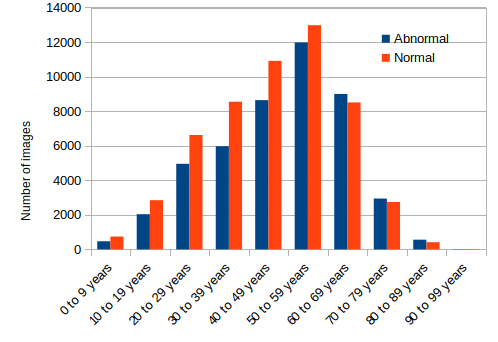
\includegraphics[width=0.48\textwidth]{images/charts/age_basic}\hspace{0.01\textwidth}%
  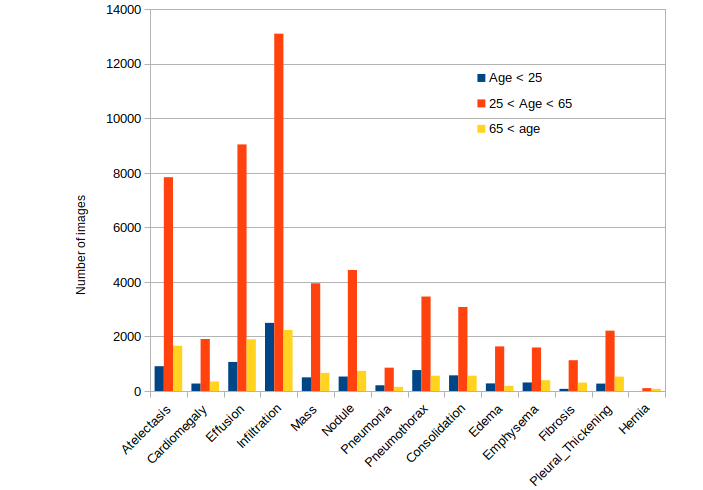
\includegraphics[width=0.48\textwidth]{images/charts/age_detailed}\\[0.01\textwidth]
  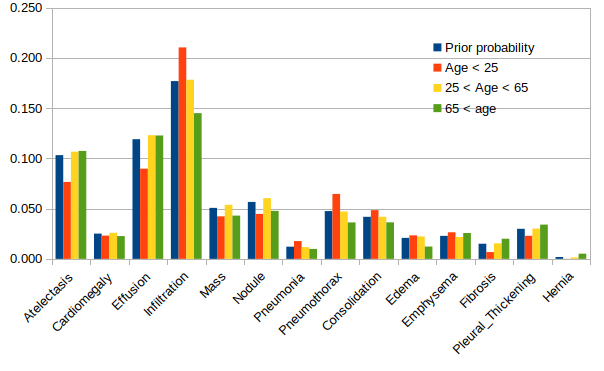
\includegraphics[width=0.48\textwidth]{images/charts/age_probs}\hspace{0.01\textwidth}%
  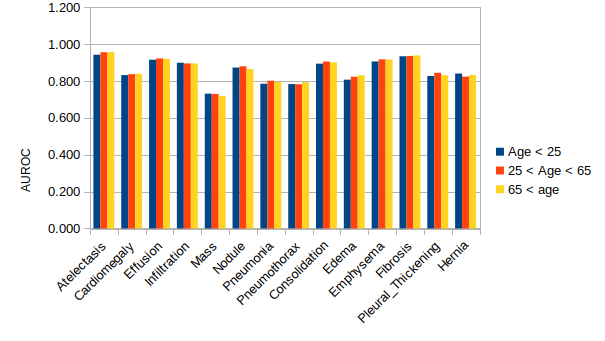
\includegraphics[width=0.48\textwidth]{images/charts/age_auc}\\[0.01\textwidth]
  \caption{Age bias. From top-left clockwise, a) distribution by age, b) distribution by age broken down by abnormality, c) baseline model's AUROC for each abnormality and d) prior and posterior probabilities of each disease given age-group.}
  % \end{minipage}
  % }
  \label{fig:age_bias}
\end{figure}

\subsection{Gender}
In the combined training and test sets of the NIH CXR-14 dataset (90\%), the male to female ratio is approximately 1.28, with similar rates of abnormality, 53.5\% and 54.1\% for males and females respectively, and \emph{No finding} is only weakly correlated with \emph{female}, with a Pearson product-moment correlation coefficient (PMCC) of 0.006.
However, when broken down by specific abnormalities, the ratio of the posterior probability of an abnormality given the gender to its prior probability shows significant variation, with \emph{Hernia} becoming 1.3 times more likely and \emph{Cardiomegaly} becoming 1.2 times more likely if the patient is female (pregnancy is a common cause of \emph{Cardiomegaly}).\\

Moreover, a similar network (with the same architecture, the only difference being 2 output nodes in the final layer instead of the 14) trained to identify gender from x-ray images on this dataset acheived an accuracy of 93.8\% (AUROC of 98.9\%) on this task when trained for a single epoch. Saliency maps showed high activations at and around regions of the image containing female breasts (as shown in figure \ref{fig:gender_bias}).\\

Although this does not necessarily mean that our abnormality-detection models are biased, the two findings above show that some bias exists in the dataset and that these models are capable of exploiting these. We evaluated our baseline model for variable performance for males and females and found that the model showed similar performance (in terms of AUROC) for both genders.

\begin{landscape}
\begin{table}
\centering
\begin{tabular}{@{}lllllllllll@{}}
\toprule
\textbf{Abnormality}        & \multicolumn{3}{l}{\textbf{Number of images}} &  \textbf{Prior} & \multicolumn{2}{l}{\textbf{Posterior}} & \multicolumn{2}{l}{\textbf{Posterior / Prior}} & \multicolumn{2}{l}{\textbf{AUROC}}       \\ \midrule
                   & Total            & Female & Male  &                   & Female                & Male  & Female            & Male & Female & Male  \\ \midrule
Atelectasis        & 10416            & 4202   & 6214  & 0.103             & 0.095                 & 0.109 & 0.92              & 1.06 & 0.951  & 0.942 \\ \midrule
Cardiomegaly       & 2532             & 1347   & 1185  & 0.025             & 0.031                 & 0.021 & 1.22              & 0.83 & 0.835  & 0.840 \\ \midrule
Effusion           & 12015            & 5311   & 6704  & 0.119             & 0.120                 & 0.118 & 1.01              & 0.99 & 0.921  & 0.923 \\ \midrule
Infiltration       & 17852            & 7622   & 10230 & 0.177             & 0.173                 & 0.180 & 0.98              & 1.02 & 0.896  & 0.896 \\ \midrule
Mass               & 5121             & 2035   & 3086  & 0.051             & 0.046                 & 0.054 & 0.91              & 1.07 & 0.732  & 0.727 \\ \midrule
Nodule             & 5710             & 2417   & 3293  & 0.057             & 0.055                 & 0.058 & 0.97              & 1.02 & 0.877  & 0.877 \\ \midrule
Pneumonia          & 1220             & 517    & 703   & 0.012             & 0.012                 & 0.012 & 0.97              & 1.02 & 0.797  & 0.803 \\ \midrule
Pneumothorax       & 4794             & 2351   & 2443  & 0.048             & 0.053                 & 0.043 & 1.12              & 0.91 & 0.771  & 0.783 \\ \midrule
Consolidation      & 4220             & 1810   & 2410  & 0.042             & 0.041                 & 0.042 & 0.98              & 1.01 & 0.907  & 0.901 \\ \midrule
Edema              & 2103             & 997    & 1106  & 0.021             & 0.023                 & 0.019 & 1.08              & 0.93 & 0.815  & 0.826 \\ \midrule
Emphysema          & 2308             & 847    & 1461  & 0.023             & 0.019                 & 0.026 & 0.84              & 1.12 & 0.919  & 0.912 \\ \midrule
Fibrosis           & 1520             & 702    & 818   & 0.015             & 0.016                 & 0.014 & 1.06              & 0.96 & 0.935  & 0.936 \\ \midrule
Pleural Thickening & 3013             & 1205   & 1808  & 0.030             & 0.027                 & 0.032 & 0.92              & 1.07 & 0.837  & 0.841 \\ \midrule
Hernia             & 186              & 106    & 80    & 0.002             & 0.002                 & 0.001 & 1.30              & 0.76 & 0.828  & 0.824 \\
\bottomrule
\end{tabular}\
\caption{Distribution by gender, and prior and posterior probabilities of each disease given the gender.}
\label{tab:gender_bias}
\end{table}
\end{landscape}

\begin{figure}[H]
  % \fbox{
  % \begin{minipage}{\textwidth}
  \centering
  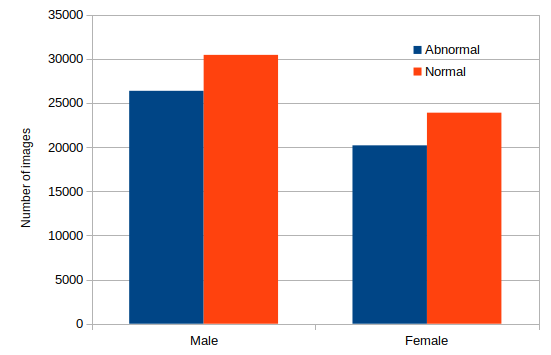
\includegraphics[width=0.48\textwidth]{images/charts/gender_basic}\hspace{0.01\textwidth}%
  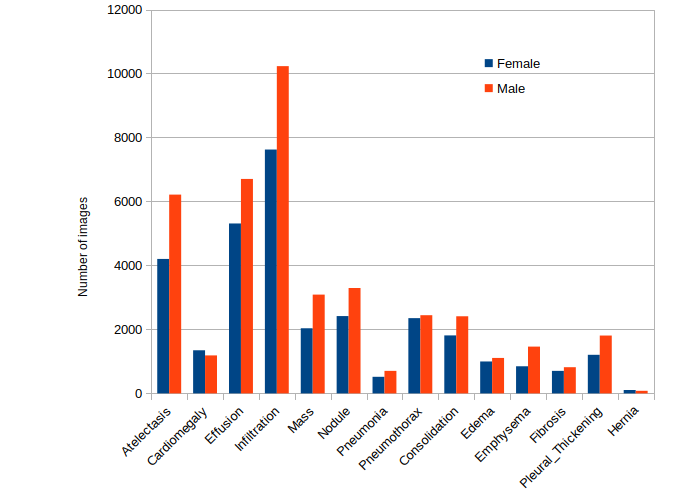
\includegraphics[width=0.48\textwidth]{images/charts/gender_detailed}\\[0.01\textwidth]
  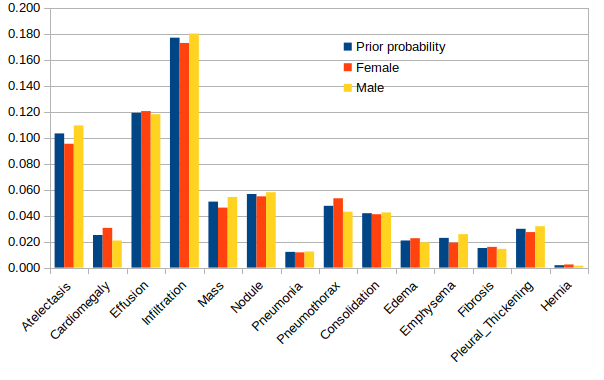
\includegraphics[width=0.48\textwidth]{images/charts/gender_probs}\hspace{0.01\textwidth}%
  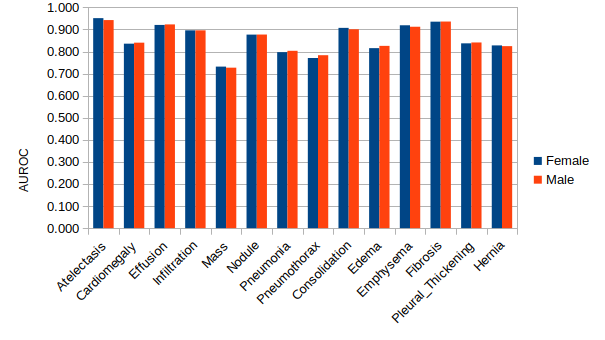
\includegraphics[width=0.48\textwidth]{images/charts/gender_auc}\\[0.01\textwidth]
  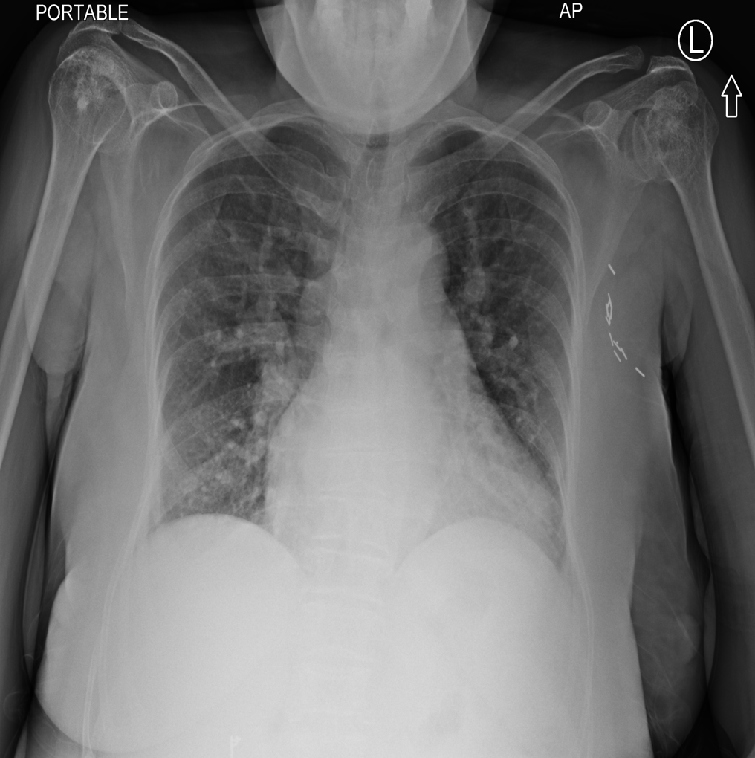
\includegraphics[width=0.48\textwidth]{images/gender_cropped_orig}\hspace{0.01\textwidth}%
  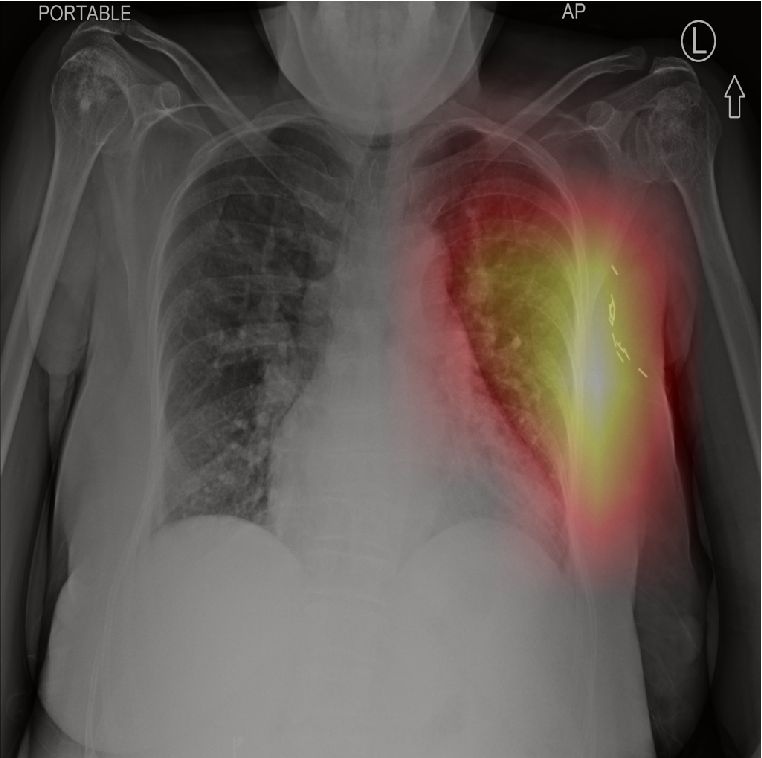
\includegraphics[width=0.48\textwidth]{images/gender_cropped}\\[0.01\textwidth]
  \caption{Gender bias. First two rows: From top-left clockwise, a) distribution by gender, b) distribution by gender broken down by abnormality, c) baseline model's AUROC for each abnormality and d) prior and posterior probabilities of each disease given gender. The $3^{rd}$ row shows saliency map for a \emph{female} prediction showing high activation around regions of the image containing female breasts.}
  % \end{minipage}
  % }
  \label{fig:gender_bias}
\end{figure}



\subsection{View-position}
The PA (posterioanterior) view is preferred over the AP (anterioposterior) view. However, the AP view is usually chosen over the PA view for younger children and is necessitated for very ill patients who cannot stand erect. The PA view is more common in the NIH CXR-14 dataset with 60\% of the images showing the PA view. Abnormality rate is higher for the AP view (52.8\%) compared to the PA view (41.6\%), and \emph{No finding} is positively correlated with PA with a Pearson product-moment correlation coefficient (PMCC) of 0.11. When broken down by specific abnormalities, the ratio of the posterior probability of an abnormality given the view-position to its prior probability shows significant variation, with \emph{Edema} and \emph{Consolidation} becoming 2.2 times and 1.7 times more likely respectively if the x-ray image shows AP view.\\

Moreover, a network with a similar architecture with 2 output nodes trained to identify the view-position from x-ray images acheived an accuracy of 98.7\% (AUROC of 99.7\%) on this task when trained for a single epoch. Saliency maps showed high activations at and around the anterior aspect of the ribs and around shadows of tokens on x-ray that identified the machine as being a \emph{portable} machine (as shown in figure \ref{fig:view_bias}).\\

We evaluated our baseline for variable performace for each view-position and found that the model showed similar performance (in terms of AUROC, sensitivity and specificity).

\begin{landscape}
\begin{table}
\centering
\begin{tabular}{@{}lllllllllll@{}}
\toprule
\textbf{Abnormality}        & \multicolumn{3}{l}{\textbf{Number of images}} &  \textbf{Prior} & \multicolumn{2}{l}{\textbf{Posterior}} & \multicolumn{2}{l}{\textbf{Posterior / Prior}} & \multicolumn{2}{l}{\textbf{AUROC}}       \\ \midrule
                   & Total & PA   & AP   &       & PA    & AP    & PA   & AP   & PA       & AP       \\ \midrule
Atelectasis        & 10416 & 5161 & 5255 & 0.103 & 0.085 & 0.130 & 0.83 & 1.26 & 0.942437 & 0.95283  \\ \midrule
Cardiomegaly       & 2532  & 1435 & 1097 & 0.025 & 0.024 & 0.027 & 0.95 & 1.08 & 0.836189 & 0.837878 \\ \midrule
Effusion           & 12015 & 5977 & 6038 & 0.119 & 0.099 & 0.149 & 0.83 & 1.25 & 0.917303 & 0.928475 \\ \midrule
Infiltration       & 17852 & 8342 & 9510 & 0.177 & 0.138 & 0.235 & 0.78 & 1.33 & 0.894947 & 0.898967 \\ \midrule
Mass               & 5121  & 3171 & 1950 & 0.051 & 0.052 & 0.048 & 1.03 & 0.95 & 0.729112 & 0.726252 \\ \midrule
Nodule             & 5710  & 3794 & 1916 & 0.057 & 0.063 & 0.047 & 1.11 & 0.84 & 0.873476 & 0.881735 \\ \midrule
Pneumonia          & 1220  & 537  & 683  & 0.012 & 0.009 & 0.017 & 0.73 & 1.40 & 0.800406 & 0.803007 \\ \midrule
Pneumothorax       & 4794  & 3056 & 1738 & 0.048 & 0.051 & 0.043 & 1.06 & 0.90 & 0.780797 & 0.797678 \\ \midrule
Consolidation      & 4220  & 1378 & 2842 & 0.042 & 0.023 & 0.070 & 0.54 & 1.68 & 0.903083 & 0.904439 \\ \midrule
Edema              & 2103  & 256  & 1847 & 0.021 & 0.004 & 0.046 & 0.20 & 2.19 & 0.824132 & 0.820317 \\ \midrule
Emphysema          & 2308  & 1359 & 949  & 0.023 & 0.022 & 0.023 & 0.98 & 1.03 & 0.914292 & 0.91912  \\ \midrule
Fibrosis           & 1520  & 1268 & 252  & 0.015 & 0.021 & 0.006 & 1.39 & 0.41 & 0.933933 & 0.934433 \\ \midrule
Pleural Thickening & 3013  & 2156 & 857  & 0.030 & 0.036 & 0.021 & 1.19 & 0.71 & 0.843553 & 0.829741 \\ \midrule
Hernia             & 186   & 159  & 27   & 0.002 & 0.003 & 0.001 & 1.43 & 0.36 & 0.828903 & 0.82359  \\
\bottomrule
\end{tabular}
\caption{Distribution by view-position, and prior and posterior probabilities of each disease given the view-position.}
\label{}
\end{table}
\end{landscape}

\begin{figure}[H]
  % \fbox{
  % \begin{minipage}{\textwidth}
  \centering
  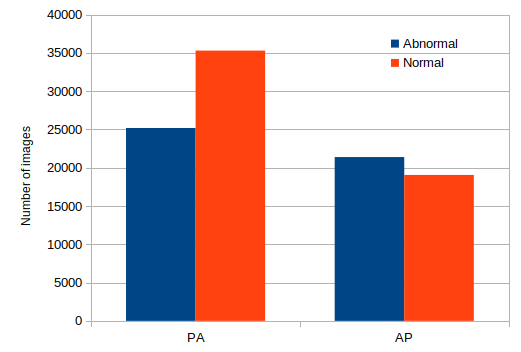
\includegraphics[width=0.48\textwidth]{images/charts/view_basic}\hspace{0.01\textwidth}%
  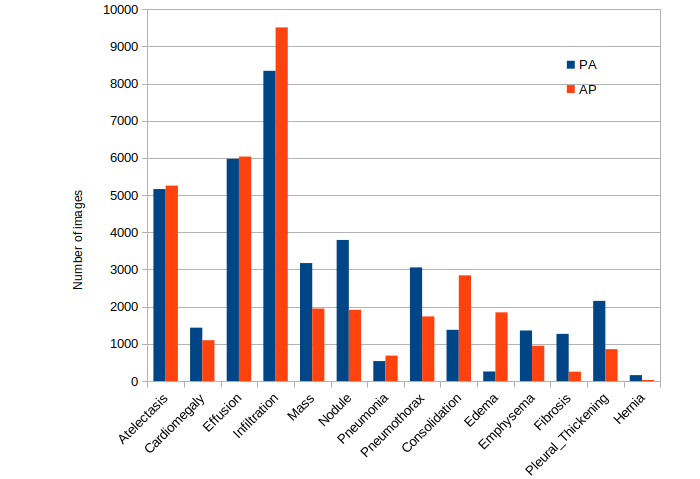
\includegraphics[width=0.48\textwidth]{images/charts/view_detailed}\\[0.01\textwidth]
  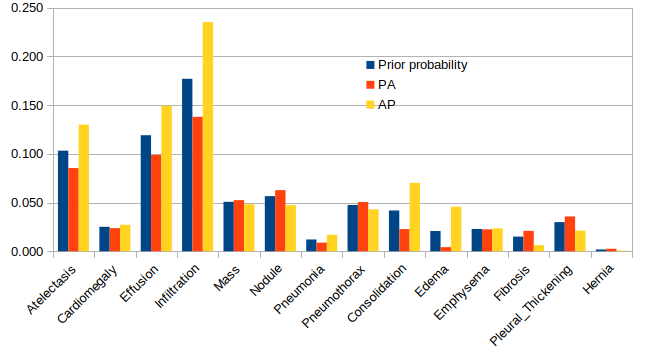
\includegraphics[width=0.48\textwidth]{images/charts/view_probs}\hspace{0.01\textwidth}%
  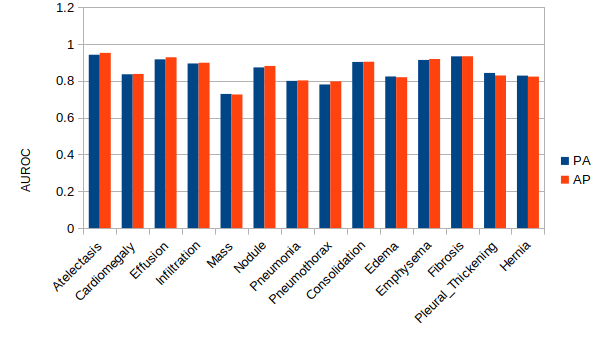
\includegraphics[width=0.48\textwidth]{images/charts/view_auc}\\[0.01\textwidth]
  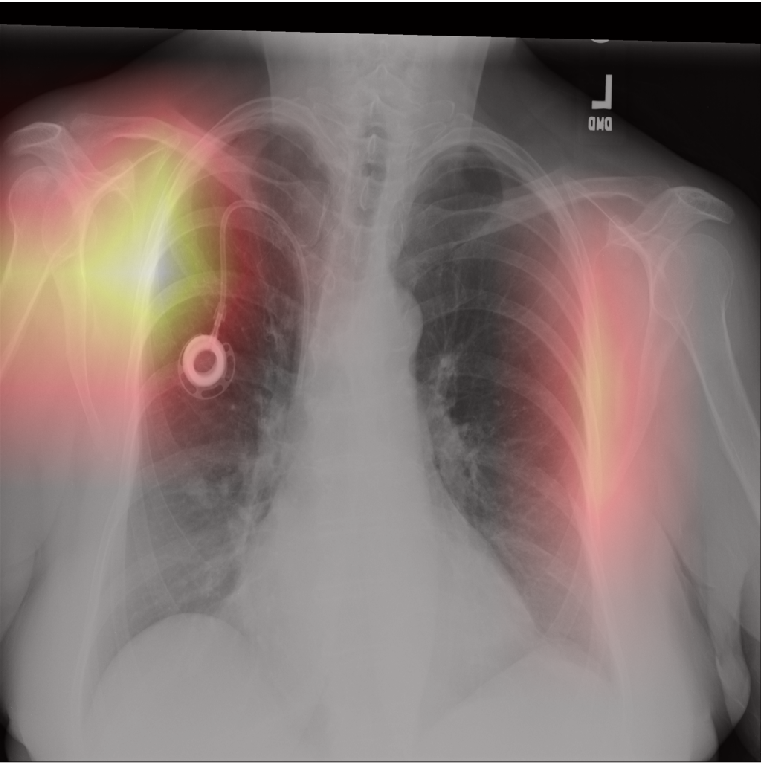
\includegraphics[width=0.48\textwidth]{images/view1_cropped}\hspace{0.01\textwidth}%
  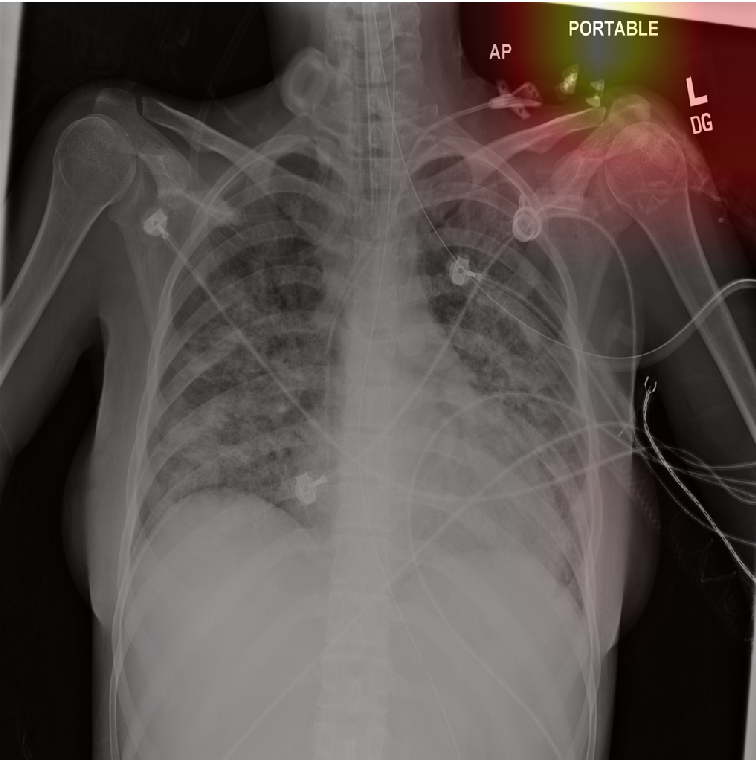
\includegraphics[width=0.48\textwidth]{images/view2_cropped}\\[0.01\textwidth]
  \caption{View bias. First two rows: From top-left clockwise, a) distribution by view-position, b) distribution by view-position broken down by abnormality, c) baseline model's AUROC for each abnormality and d) prior and posterior probabilities of each disease given view-position. The $3^{rd}$ from left to right shows saliency maps for \emph{PA} and \emph{AP} showing high activation at and around the anterior aspect of the ribs and around shadows of tokens on the x-ray identifying the machine as being a \emph{portable} machine.}
  % \end{minipage}
  % }
  \label{fig:view_bias}
\end{figure}

\section{Generalization}
We evaluate the ability of our baselines to generalize to other hospital
systems. At the problem of pneumonia detection, we train on the NIH CXR-14
dataset and test on both the internal test set and the external Guangzhou
dataset, a pediatric pneumonia dataset from a different hospital system.\\

At the problem of tuberculosis detection, we train on the Shenzhen tuberculosis
and and test on both the internal test set and the external Montgomery
tuberculosis
dataset from a different hospital system.\\

We find that the baseline model trained to detect pneumonia on the NIH CXR-14
dataset performs better on the Guangzhou dataset than the internal test set but
worse that a model trained exclusively on the external dataset, and the baseline
model trained to detect tuberculosis on the Shenzhen dataset shows inferior
performace on the external dataset, but which is better than a model trained
exclusively on the external dataset.

\begin{table}[]
  \centering
  \begin{tabular}{@{}llll@{}}
    \toprule
    \textbf{}                              & \textbf{Training} & \textbf{Testing} & \textbf{AUROC} \\ \midrule
    \multirow{3}{*}{\textbf{Pneumonia}}    & NIH CXR-14        & NIH CXR-14       & 0.760                                                                            \\ \cmidrule(l){2-4} 
                                           & NIH CXR-14        & Guangzhou   & 0.842                                                                           \\ \cmidrule(l){2-4} 
                                           & Guangzhou    & Guangzhou   & 0.9                                                                            \\ \midrule
    \multirow{3}{*}{\textbf{Tuberculosis}} & Shenzhen          & Shenzhen         & 0.956                                                                            \\ \cmidrule(l){2-4} 
                                           & Shenzhen          & Montgomery       & 0.871                                                                           \\ \cmidrule(l){2-4} 
                                           & Montgomery        & Montgomery       & 0.631                                                                            \\ \bottomrule
  \end{tabular}
  \caption{Evaluation results for our baseline models' ability to generalize to
    external datasets}
  \label{tab:generalization}
\end{table}

\section{Viral and bacterial pneumonia}
Images in the Guangzhou pediatric pneumonia dataset that show manifestations
of pneumonia are further categorized as \emph{Viral} and \emph{bacterial}.
Since viral and bacterial pneumonia present different levels of emergency and warrant
different courses of treatment, we evaluate our models for variable performance on these
categories to ensure that they are not biased toward one or the other type.\\

We found that the models trained on the NIH CXR-14 dataset were better at
detecting viral pneumonia than bacterial pneumonia.

\begin{table}[]
  \centering
  \begin{tabular}{@{}lll@{}}
    \toprule
    \textbf{Model}                        & \multicolumn{2}{l}{\textbf{AUROC}}  \\ \midrule
    \textbf{}                             & Bacterial pneumonia                             & Viral pneumonia \\ \midrule
    Baseline                              & 0.835                                           & \textbf{0.855}                  \\ \midrule
    Higher resolution (512 x 512)         & 0.816                                           & \textbf{0.821}                  \\ \midrule
    Progressive resizing (upto 512 x 512) & 0.860                                           & \textbf{0.891}                  \\ \midrule
    Mixup, with $\alpha = 0.4$            & 0.860                                           & \textbf{0.895}                  \\ \bottomrule
  \end{tabular}
  \caption{Variable performance on viral and bacterial pneumonia of models trained on the NIH CXR-14 dataset.}
  \label{tab:viral_vs_bacterial}
\end{table}

\section{Segmentation and centering}
The Montgomery dataset includes hand-annotated segmentation masks of both the left and right lungs for each image. We evaluate models trained on the Shenzhen hospital tuberculosis dataset, on the Montgmomery dataset after a) segmenting the lung regions and b) segmeting the lung regions and cropping to the smallest rectangle which encloses both the lungs.\\

Across multiple models and trials and averaged across 9 folds, we failed to see a significant increase or decrease in performance among models trained on un-segmented images, segmented images and segmented and cropped images.

\begin{table}
\centering
\begin{tabular}{@{}llll@{}}
\toprule
\textbf{Model}         & \textbf{Average AUROC} &           & \\
\midrule
                       & Un-segmented           & Segmented & Segmented and cropped \\
\midrule
Baseline (224 x 224)   & 0.871                  & 0.867     & 0.874                 \\
(320 x 320)            & 0.846                  & 0.854     & 0.859                 \\
(448 x 448)            & 0.809                  & 0.811     & 0.795                 \\
(540 x 540)            & 0.828                  & 0.826     & 0.812                 \\
(672 x 672)            & 0.813                  & 0.814     & 0.828                 \\
(224 x 224) Pretrained & 0.941                  & 0.940     & 0.942                 \\
(480 x 480) Pretrained & 0.957                  & 0.957     & 0.955                 \\
\bottomrule
\end{tabular}
\caption{Performance of models trained on the Shenzhen dataset and evaluated on the Montgomery dataset without segmentation, with segmentation and with segmentation and cropping.}
  \label{tab:mc_segmentation}
\end{table}

\chapter{Results\label{res}}
\section{Comparison to previous work and human radiologists}
For the NIH CXR-14 dataset, we achieve performance competitive with previous
work and show improvements over our baseline. See table \ref{tab:nih_previous} for
the results. Rajpurkar et al. in \cite{Rajpurkar2018a} measured human
performance in terms of AUROC for each disease, using the majority vote of 3
independent board-certified cardiothoracic specialist radiologists (average
experience 15 years) as ground truth, and measure the the performance of 6 BC
radiologists from 3 academic institutions (average experience 12 years) and 3
senior radiology residents by fitting a curve to these 9 radiologists' operating
points and calculating the area under it. We compare our models with human
radiologist performance and find that the model's performance is on average
within 2\% of that of human radiologists (see table
\ref{tab:nih_comparision} for the comparison).\\

On the Shenzhen and Montgomery datasets, we achieve performance comparable to
previous work and show improvement over our baseline. See tables
\ref{tab:shenzhen_previous} and \ref{tab:montgomery_previous} for the results.

\begin{table}[]
  \centering
  \begin{tabular}{ll}
    \hline
    \textbf{Authors}            & \textbf{Average AUROC} \\ \hline
    Wang et al. (2017)          & 0.738                  \\ \hline
    Y. Shen et al.              & 0.775                  \\ \hline
    H. Wang et al. (ChestNet)   & 0.781                  \\ \hline
    P. Kumar et al.             & 0.792                  \\ \hline
    Yao et al. (2017)           & 0.803                  \\ \hline
    Y. Tang et al.              & 0.805                  \\ \hline
    S. Guendel et al.           & 0.807                  \\ \hline
    Yan et al.                  & 0.83                   \\ \hline
    X. Xu et al. (DeepCXray)    & 0.832                  \\ \hline
    Rajpurkar et al. (CheXNet)  & 0.841                  \\ \hline
    B. Zhou et al.              & 0.842                  \\ \hline
    Rajpurkar et al. (ChexNext) & 0.849                  \\ \hline
    \textbf{Our model}          & \textbf{0.856}         \\ \hline
    Q. Guan et al.              & 0.871                  \\ \hline
  \end{tabular}
  \caption{Comparison to previous work on the NIH CXR-14 dataset}
  \label{tab:nih_previous}
\end{table}

\begin{table}[]
  \centering
  \begin{tabular}{lllll}
    \hline
    \textbf{Abnormality} & \multicolumn{4}{l}{\textbf{AUROC}}             \\ \hline
                         & Baseline & Ensemble & Radiologist & Difference (\%) \\ \hline
    Atelectasis          & 0.823    & 0.839    & 0.808       & -3.06      \\ \hline
    Cardiomegaly         & 0.899    & 0.916    & 0.888       & -2.79      \\ \hline
    Effusion             & 0.881    & 0.89     & 0.9         & 0.96       \\ \hline
    Infiltration         & 0.705    & 0.72     & 0.734       & 1.39       \\ \hline
    Mass                 & 0.857    & 0.868    & 0.886       & 1.76       \\ \hline
    Nodule               & 0.779    & 0.817    & 0.899       & 8.17       \\ \hline
    Pneumonia            & 0.767    & 0.765    & 0.823       & 5.83       \\ \hline
    Pneumothorax         & 0.881    & 0.895    & 0.94        & 4.46       \\ \hline
    Consolidation        & 0.822    & 0.819    & 0.841       & 2.22       \\ \hline
    Edema                & 0.911    & 0.902    & 0.91        & 0.83       \\ \hline
    Emphysema            & 0.913    & 0.944    & 0.911       & -3.33      \\ \hline
    Fibrosis             & 0.824    & 0.854    & 0.897       & 4.31       \\ \hline
    Pleural Thickening  & 0.81     & 0.805    & 0.779       & -2.59      \\ \hline
    Hernia               & 0.906    & 0.944    & 0.985       & 4.1        \\ \hline
    \textbf{Average}              & \textbf{0.841}    & \textbf{0.856}    & \textbf{0.8715}      & \textbf{1.59}       \\ \hline
  \end{tabular}
  \caption{Comparison to human radiologists on the NIH CXR-14 dataset}
  \label{tab:nih_comparision}
\end{table}

\begin{table}[]
  \centering
  \begin{tabular}{lll}
    \hline
    \textbf{Authors}                    & \textbf{AUROC} &\textbf{Accuracy}\\ \hline
    Jaeger et al                        & 0.9            & 0.841\\ \hline
    Hwang et al                         & 0.93           & 0.837\\ \hline
    Lopez and Valiati                   & 0.926          & 0.846\\ \hline
    MT Islam et al                      & 0.94           & 0.9\\ \hline
    Haloi et al                         & 0.949          & \\ \hline
    Liu et al (ResNet-152)              & 0.967          & 0.923\\ \hline
    Liu et al (Inception-ResNet-v2)     & 0.983          & 0.917\\ \hline
    Vajda et al                         & 0.99           & 0.957\\ \hline
    \textbf{Our baseline}               & \textbf{0.956} & \textbf{0.902}        \\ \hline
    \textbf{\begin{tabular}[c]{@{}l@{}}Our best model\\ Pretrained on NIH CXR-14\\ with mixup $\alpha = 0.4$\end{tabular}} & \textbf{0.985}          & \textbf{0.949}\\ \hline
  \end{tabular}
  \caption{Comparison to previous work on the Shenzhen tuberculosis dataset}
  \label{tab:shenzhen_previous}
\end{table}

\begin{table}[]
  \centering
  \begin{tabular}{lll}
    \hline
    \textbf{Authors}                   & \textbf{AUROC}  & \textbf{Accuracy}\\ \hline
    Jaeger et al                       & 0.869           & 0.783 \\ \hline
    Lopez and Valiati                  & 0.926           & 0.826 \\ \hline
    Liu et al (Inception-ResNet-v2)    & 0.957           & 0.844 \\ \hline
    Liu et al (ResNet-152)             & 0.951           & 0.890 \\ \hline
    Vajda et al                        & 0.870           & 0.783 \\ \hline
    \textbf{Our baseline}              & \textbf{0.871}  & \textbf{0.755}\\ \hline
    \textbf{\begin{tabular}[c]{@{}l@{}}Our best model\\ Pre-trained on NIH CXR-14\\ (480 x 480)\end{tabular}} & \textbf{0.957} & \textbf{0.89}\\ \hline
  \end{tabular}
  \caption{Comparison to previous work on the Montgomery tuberculosis dataset}
  \label{tab:montgomery_previous}
\end{table}

% \subsection{Caveats with comparison to human radiologists}
% \section{Other important factors}
% Such as how well predicted probabilities correspond to actual severity,
% localization, and time
\section{Examples}

\begin{figure}[H]
  % \fbox{
  % \begin{minipage}{\textwidth}
  \centering
  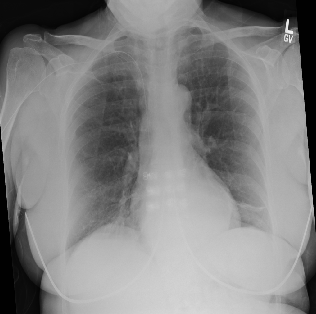
\includegraphics[width=0.3\textwidth]{images/preds/atelectasis}\hspace{0.01\textwidth}%
  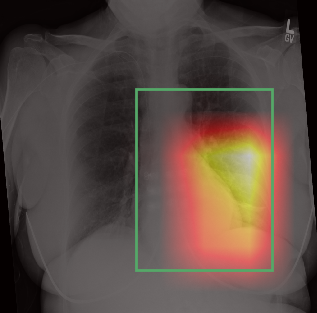
\includegraphics[width=0.3\textwidth]{images/preds/atelectasis_cam}\hspace{0.01\textwidth}%
  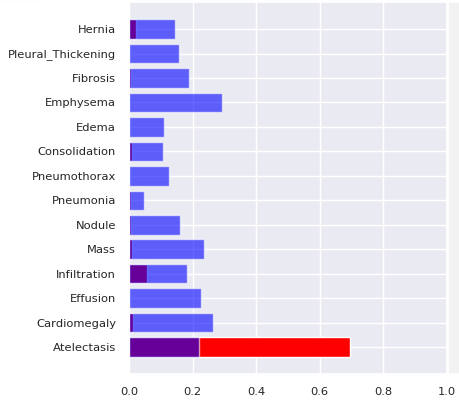
\includegraphics[width=0.3\textwidth]{images/preds/atelectasis_probs}\\[0.01\textwidth]
  \caption{Original image, image overlaid with saliency map and bounding boxes
    for \emph{Atelectasis}, and predicted probabilities for an x-ray image.}
  % \end{minipage}
  % }
  \label{examples_1}
\end{figure}
\begin{figure}[H]
  % \fbox{
  % \begin{minipage}{\textwidth}
  \centering
  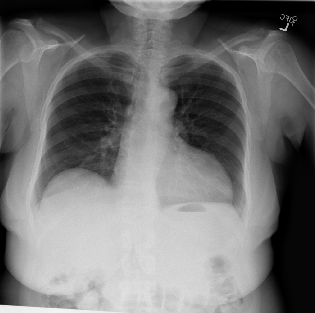
\includegraphics[width=0.3\textwidth]{images/preds/cardiomegaly}\hspace{0.01\textwidth}%
  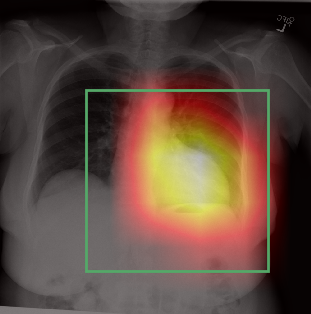
\includegraphics[width=0.3\textwidth]{images/preds/cardiomegaly_cam}\hspace{0.01\textwidth}%
  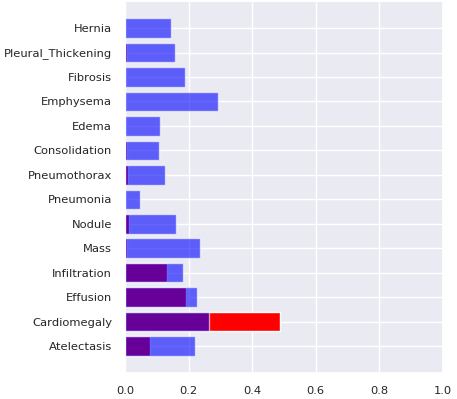
\includegraphics[width=0.3\textwidth]{images/preds/cardiomegaly_probs}\\[0.01\textwidth]
  \caption{Original image, image overlaid with saliency map and bounding boxes
    for \emph{Cardiomegaly}, and predicted probabilities for an x-ray image.}
  % \end{minipage}
  % }
  \label{examples_2}
\end{figure}

\begin{figure}[H]
  % \fbox{
  % \begin{minipage}{\textwidth}
  \centering
  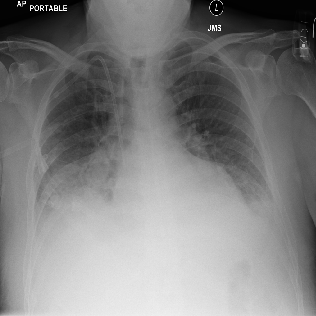
\includegraphics[width=0.3\textwidth]{images/preds/effusion}\hspace{0.01\textwidth}%
  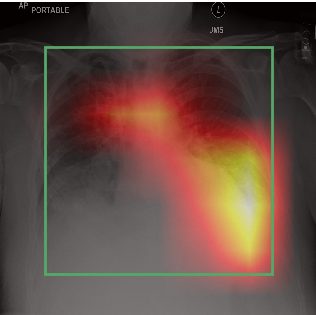
\includegraphics[width=0.3\textwidth]{images/preds/effusion_cam}\hspace{0.01\textwidth}%
  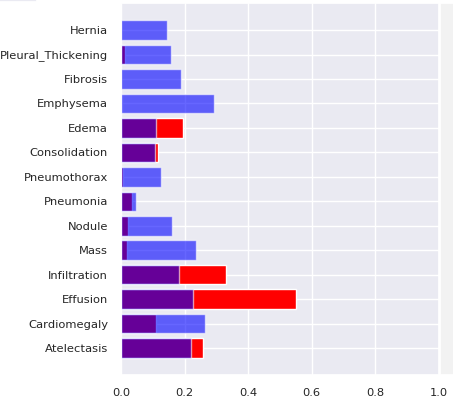
\includegraphics[width=0.3\textwidth]{images/preds/effusion_probs}\\[0.01\textwidth]
  \caption{Original image, image overlaid with saliency map and bounding boxes
    for \emph{Effusion}, and predicted probabilities for an x-ray image.}
  % \end{minipage}
  % }
  \label{examples_3}
\end{figure}

\begin{figure}[H]
  % \fbox{
  % \begin{minipage}{\textwidth}
  \centering
  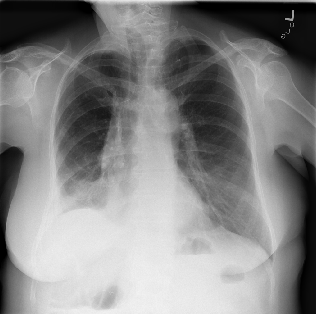
\includegraphics[width=0.3\textwidth]{images/preds/infiltration}\hspace{0.01\textwidth}%
  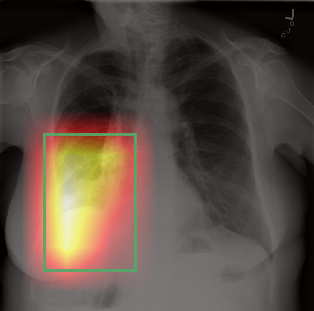
\includegraphics[width=0.3\textwidth]{images/preds/infiltration_cam}\hspace{0.01\textwidth}%
  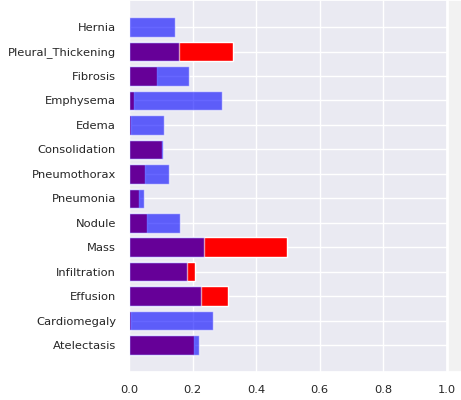
\includegraphics[width=0.3\textwidth]{images/preds/infiltration_probs}\\[0.01\textwidth]
  \caption{Original image, image overlaid with saliency map and bounding boxes
    for \emph{Infiltration}, and predicted probabilities for an x-ray image.}
  % \end{minipage}
  % }
  \label{examples_4}
\end{figure}

\begin{figure}[H]
  % \fbox{
  % \begin{minipage}{\textwidth}
  \centering
  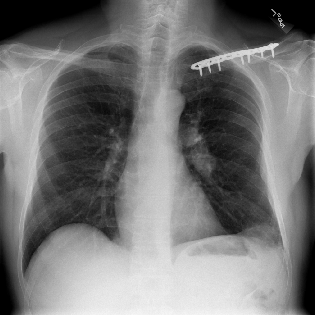
\includegraphics[width=0.3\textwidth]{images/preds/mass}\hspace{0.01\textwidth}%
  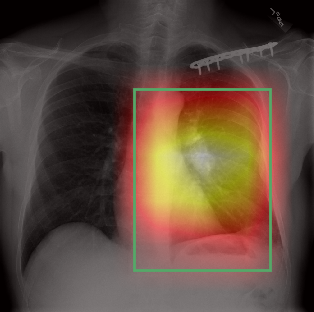
\includegraphics[width=0.3\textwidth]{images/preds/mass_cam}\hspace{0.01\textwidth}%
  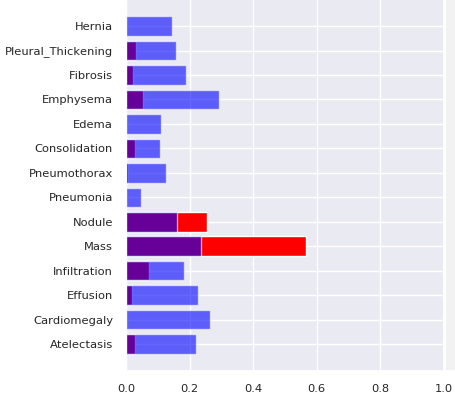
\includegraphics[width=0.3\textwidth]{images/preds/mass_probs}\\[0.01\textwidth]
  \caption{Original image, image overlaid with saliency map and bounding boxes
    for \emph{Mass}, and predicted probabilities for an x-ray image.}
  % \end{minipage}
  % }
  \label{examples_5}
\end{figure}

\begin{figure}[H]
  % \fbox{
  % \begin{minipage}{\textwidth}
  \centering
  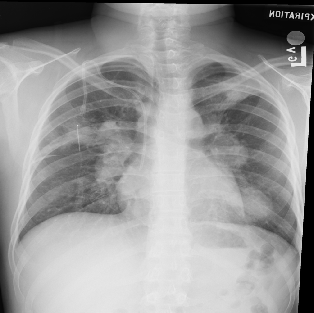
\includegraphics[width=0.3\textwidth]{images/preds/nodule}\hspace{0.01\textwidth}%
  \includegraphics[width=0.3\textwidth]{images/preds/nodule_cam}\hspace{0.01\textwidth}%
  \includegraphics[width=0.3\textwidth]{images/preds/nodule_probs}\\[0.01\textwidth]
  \caption{Original image, image overlaid with saliency map and bounding boxes
    for \emph{Nodule}, and predicted probabilities for an x-ray image.}
  % \end{minipage}
  % }
  \label{examples_6}
\end{figure}

\begin{figure}[H]
  % \fbox{
  % \begin{minipage}{\textwidth}
  \centering
  \includegraphics[width=0.3\textwidth]{images/preds/pneumonia}\hspace{0.01\textwidth}%
  \includegraphics[width=0.3\textwidth]{images/preds/pneumonia_cam}\hspace{0.01\textwidth}%
  \includegraphics[width=0.3\textwidth]{images/preds/pneumonia_probs}\\[0.01\textwidth]
  \caption{Original image, image overlaid with saliency map and bounding boxes
    for \emph{Pneumonia}, and predicted probabilities for an x-ray image.}
  % \end{minipage}
  % }
  \label{examples_7}
\end{figure}

\begin{figure}[H]
  % \fbox{
  % \begin{minipage}{\textwidth}
  \centering
  \includegraphics[width=0.3\textwidth]{images/preds/pneumothorax}\hspace{0.01\textwidth}%
  \includegraphics[width=0.3\textwidth]{images/preds/pneumothorax_cam}\hspace{0.01\textwidth}%
  \includegraphics[width=0.3\textwidth]{images/preds/pneumothorax_probs}\\[0.01\textwidth]
  \caption{Original image, image overlaid with saliency map and bounding boxes
    for \emph{Pneumothorax}, and predicted probabilities for an x-ray image.}
  % \end{minipage}
  % }
  \label{examples_8}
\end{figure}

\begin{figure}[H]
  % \fbox{
  % \begin{minipage}{\textwidth}
  \centering
  \includegraphics[width=0.3\textwidth]{images/preds/consolidation}\hspace{0.01\textwidth}%
  \includegraphics[width=0.3\textwidth]{images/preds/consolidation_cam}\hspace{0.01\textwidth}%
  \includegraphics[width=0.3\textwidth]{images/preds/consolidation_probs}\\[0.01\textwidth]
  \caption{Original image, image overlaid with saliency map and bounding boxes
    for \emph{Consolidation}, and predicted probabilities for an x-ray image.}
  % \end{minipage}
  % }
  \label{examples_9}
\end{figure}

\begin{figure}[H]
  % \fbox{
  % \begin{minipage}{\textwidth}
  \centering
  \includegraphics[width=0.3\textwidth]{images/preds/edema}\hspace{0.01\textwidth}%
  \includegraphics[width=0.3\textwidth]{images/preds/edema_cam}\hspace{0.01\textwidth}%
  \includegraphics[width=0.3\textwidth]{images/preds/edema_probs}\\[0.01\textwidth]
  \caption{Original image, image overlaid with saliency map and bounding boxes
    for \emph{Edema}, and predicted probabilities for an x-ray image.}
  % \end{minipage}
  % }
  \label{examples_10}
\end{figure}

\begin{figure}[H]
  % \fbox{
  % \begin{minipage}{\textwidth}
  \centering
  \includegraphics[width=0.3\textwidth]{images/preds/emphysema}\hspace{0.01\textwidth}%
  \includegraphics[width=0.3\textwidth]{images/preds/emphysema_cam}\hspace{0.01\textwidth}%
  \includegraphics[width=0.3\textwidth]{images/preds/emphysema_probs}\\[0.01\textwidth]
  \caption{Original image, image overlaid with saliency map and bounding boxes
    for \emph{Emphysema}, and predicted probabilities for an x-ray image.}
  % \end{minipage}
  % }
  \label{examples_11}
\end{figure}

\begin{figure}[H]
  % \fbox{
  % \begin{minipage}{\textwidth}
  \centering
  \includegraphics[width=0.3\textwidth]{images/preds/fibrosis}\hspace{0.01\textwidth}%
  \includegraphics[width=0.3\textwidth]{images/preds/fibrosis_cam}\hspace{0.01\textwidth}%
  \includegraphics[width=0.3\textwidth]{images/preds/fibrosis_probs}\\[0.01\textwidth]
  \caption{Original image, image overlaid with saliency map and bounding boxes
    for \emph{Fibrosis}, and predicted probabilities for an x-ray image.}
  % \end{minipage}
  % }
  \label{examples_12}
\end{figure}

\begin{figure}[H]
  % \fbox{
  % \begin{minipage}{\textwidth}
  \centering
  \includegraphics[width=0.3\textwidth]{images/preds/PT}\hspace{0.01\textwidth}%
  \includegraphics[width=0.3\textwidth]{images/preds/PT_cam}\hspace{0.01\textwidth}%
  \includegraphics[width=0.3\textwidth]{images/preds/PT_probs}\\[0.01\textwidth]
  \caption{Original image, image overlaid with saliency map and bounding boxes
    for \emph{Pleural Thickening}, and predicted probabilities for an x-ray
    image.}
  % \end{minipage}
  % }
  \label{examples_13}
\end{figure}

\begin{figure}[H]
  % \fbox{
  % \begin{minipage}{\textwidth}
  \centering
  \includegraphics[width=0.3\textwidth]{images/preds/hernia}\hspace{0.01\textwidth}%
  \includegraphics[width=0.3\textwidth]{images/preds/hernia_cam}\hspace{0.01\textwidth}%
  \includegraphics[width=0.3\textwidth]{images/preds/hernia_probs}\\[0.01\textwidth]
  \caption{Original image, image overlaid with saliency map and bounding boxes
    for \emph{Hernia}, and predicted probabilities for an x-ray image.}
  % \end{minipage}
  % }
  \label{examples_14}
\end{figure}

\begin{figure}[H]
  % \fbox{
  % \begin{minipage}{\textwidth}
  \centering
  \includegraphics[width=0.3\textwidth]{images/preds/no_finding}\hspace{0.01\textwidth}%
  \includegraphics[width=0.3\textwidth]{images/preds/no_finding_cam}\hspace{0.01\textwidth}%
  \includegraphics[width=0.3\textwidth]{images/preds/no_finding_probs}\\[0.01\textwidth]
  \caption{Original image, image overlaid with saliency map and bounding boxes,
    and predicted probabilities for an x-ray image showing no abnormalities.}
  % \end{minipage}
  % }
  \label{examples_15}
\end{figure}

\begin{figure}[H]
  % \fbox{
  % \begin{minipage}{\textwidth}
  \centering
  \includegraphics[width=0.45\textwidth]{images/preds/TB}\hspace{0.01\textwidth}%
  \includegraphics[width=0.45\textwidth]{images/preds/TB_cam}\\[0.01\textwidth]
  \caption{Original image, image overlaid with saliency map and bounding boxes
    for \emph{Tuberculosis}}
  % \end{minipage}
  % }
  \label{examples_16}
\end{figure}

\begin{figure}[H]
  % \fbox{
  % \begin{minipage}{\textwidth}
  \centering
  \includegraphics[width=0.45\textwidth]{images/preds/TB2}\hspace{0.01\textwidth}%
  \includegraphics[width=0.45\textwidth]{images/preds/TB2_cam}\\[0.01\textwidth]
  \caption{Original image, image overlaid with saliency map and bounding boxes
    for \emph{Tuberculosis}}
  % \end{minipage}
  % }
  \label{examples_17}
\end{figure}



\chapter{Conclusion}
We developed algorithms that can detect abnormalities on the x-ray and explain
these detections by generating heatmaps pointing out areas of the image that
most influenced it. We established baselines, benchmarked against previous work
and showed that a) transfer-learning from a large non-TB dataset dramatically
improves TB detection, b) models in the domain show inferior performance on
external data from a different hospital system but c) recent techniques such as
mixup and progressive resizing improve performance and generalization. We
achieved performance competitive with previous work in detecting pneumonia-like
and other abnormalities on the NIH chestX-ray14 dataset and in detecting
tuberculosis on the Shenzhen hospital dataset, and achieved state-of-the-art
performance on the Montgomery county tuberculosis dataset.\\

Avenues for future research include:
\begin{enumerate}
\item{Training on images from multiple hospital systems to improve the model's
    ability to generalize to other hospital systems and machine types, perhaps
    using techiniques in domain adaptation or deep domain confusion
    \cite{tzeng2014deep} to prevent the model from learning features that are
    necessary to identify the hospital system. }
\item{Exploring ways to infuse domain knowledge into the algorithm to exploit
    correlations between the abnormalities.}
\item{Using attention to allow the network to focus on pathological areas.}
\item{Training models end-to-end to generate radiology reports in natural
    language from x-ray images.}
\item{Segmentation of lung regions and bone shadow suppression to reduce the
    number of false-positives.}
\item{Using recently released datasets such as CheXPert\cite{Irvin2019} and
    PadChest\cite{Bustos2019} which have more images and a hierarchical labeling
    schema.}
\end{enumerate}
\printbibliography
\end{document}
